\documentclass[twoside]{book}

% Packages required by doxygen
\usepackage{fixltx2e}
\usepackage{calc}
\usepackage{doxygen}
\usepackage[export]{adjustbox} % also loads graphicx
\usepackage{graphicx}
\usepackage[utf8]{inputenc}
\usepackage{makeidx}
\usepackage{multicol}
\usepackage{multirow}
\PassOptionsToPackage{warn}{textcomp}
\usepackage{textcomp}
\usepackage[nointegrals]{wasysym}
\usepackage[table]{xcolor}

% Font selection
\usepackage[T1]{fontenc}
\usepackage[scaled=.90]{helvet}
\usepackage{courier}
\usepackage{amssymb}
\usepackage{sectsty}
\renewcommand{\familydefault}{\sfdefault}
\allsectionsfont{%
  \fontseries{bc}\selectfont%
  \color{darkgray}%
}
\renewcommand{\DoxyLabelFont}{%
  \fontseries{bc}\selectfont%
  \color{darkgray}%
}
\newcommand{\+}{\discretionary{\mbox{\scriptsize$\hookleftarrow$}}{}{}}

% Page & text layout
\usepackage{geometry}
\geometry{%
  a4paper,%
  top=2.5cm,%
  bottom=2.5cm,%
  left=2.5cm,%
  right=2.5cm%
}
\tolerance=750
\hfuzz=15pt
\hbadness=750
\setlength{\emergencystretch}{15pt}
\setlength{\parindent}{0cm}
\setlength{\parskip}{3ex plus 2ex minus 2ex}
\makeatletter
\renewcommand{\paragraph}{%
  \@startsection{paragraph}{4}{0ex}{-1.0ex}{1.0ex}{%
    \normalfont\normalsize\bfseries\SS@parafont%
  }%
}
\renewcommand{\subparagraph}{%
  \@startsection{subparagraph}{5}{0ex}{-1.0ex}{1.0ex}{%
    \normalfont\normalsize\bfseries\SS@subparafont%
  }%
}
\makeatother

% Headers & footers
\usepackage{fancyhdr}
\pagestyle{fancyplain}
\fancyhead[LE]{\fancyplain{}{\bfseries\thepage}}
\fancyhead[CE]{\fancyplain{}{}}
\fancyhead[RE]{\fancyplain{}{\bfseries\leftmark}}
\fancyhead[LO]{\fancyplain{}{\bfseries\rightmark}}
\fancyhead[CO]{\fancyplain{}{}}
\fancyhead[RO]{\fancyplain{}{\bfseries\thepage}}
\fancyfoot[LE]{\fancyplain{}{}}
\fancyfoot[CE]{\fancyplain{}{}}
\fancyfoot[RE]{\fancyplain{}{\bfseries\scriptsize Generated by Doxygen }}
\fancyfoot[LO]{\fancyplain{}{\bfseries\scriptsize Generated by Doxygen }}
\fancyfoot[CO]{\fancyplain{}{}}
\fancyfoot[RO]{\fancyplain{}{}}
\renewcommand{\footrulewidth}{0.4pt}
\renewcommand{\chaptermark}[1]{%
  \markboth{#1}{}%
}
\renewcommand{\sectionmark}[1]{%
  \markright{\thesection\ #1}%
}

% Indices & bibliography
\usepackage{natbib}
\usepackage[titles]{tocloft}
\setcounter{tocdepth}{3}
\setcounter{secnumdepth}{5}
\makeindex

% Hyperlinks (required, but should be loaded last)
\usepackage{ifpdf}
\ifpdf
  \usepackage[pdftex,pagebackref=true]{hyperref}
\else
  \usepackage[ps2pdf,pagebackref=true]{hyperref}
\fi
\hypersetup{%
  colorlinks=true,%
  linkcolor=blue,%
  citecolor=blue,%
  unicode%
}

% Custom commands
\newcommand{\clearemptydoublepage}{%
  \newpage{\pagestyle{empty}\cleardoublepage}%
}

\usepackage{caption}
\captionsetup{labelsep=space,justification=centering,font={bf},singlelinecheck=off,skip=4pt,position=top}

%===== C O N T E N T S =====

\begin{document}

% Titlepage & ToC
\hypersetup{pageanchor=false,
             bookmarksnumbered=true,
             pdfencoding=unicode
            }
\pagenumbering{alph}
\begin{titlepage}
\vspace*{7cm}
\begin{center}%
{\Large My Project }\\
\vspace*{1cm}
{\large Generated by Doxygen 1.8.13}\\
\end{center}
\end{titlepage}
\clearemptydoublepage
\pagenumbering{roman}
\tableofcontents
\clearemptydoublepage
\pagenumbering{arabic}
\hypersetup{pageanchor=true}

%--- Begin generated contents ---
\chapter{R\+E\+A\+D\+ME}
\label{md_README}
\Hypertarget{md_README}
\#\+Projet Yahtzee Repertoire pour le projet de jeu Yahtzee 
\chapter{Data Structure Index}
\section{Data Structures}
Here are the data structures with brief descriptions\+:\begin{DoxyCompactList}
\item\contentsline{section}{\hyperlink{structPlayer}{Player} }{\pageref{structPlayer}}{}
\end{DoxyCompactList}

\chapter{File Index}
\section{File List}
Here is a list of all files with brief descriptions\+:\begin{DoxyCompactList}
\item\contentsline{section}{\hyperlink{affichage_8c}{affichage.\+c} }{\pageref{affichage_8c}}{}
\item\contentsline{section}{\hyperlink{header_8h}{header.\+h} }{\pageref{header_8h}}{}
\item\contentsline{section}{\hyperlink{main_8c}{main.\+c} }{\pageref{main_8c}}{}
\item\contentsline{section}{\hyperlink{mecanismeJeu_8c}{mecanisme\+Jeu.\+c} }{\pageref{mecanismeJeu_8c}}{}
\item\contentsline{section}{\hyperlink{mecanismeJeu_8h}{mecanisme\+Jeu.\+h} }{\pageref{mecanismeJeu_8h}}{}
\item\contentsline{section}{\hyperlink{proto_8c}{proto.\+c} }{\pageref{proto_8c}}{}
\item\contentsline{section}{\hyperlink{score_8c}{score.\+c} }{\pageref{score_8c}}{}
\item\contentsline{section}{\hyperlink{score_8h}{score.\+h} }{\pageref{score_8h}}{}
\item\contentsline{section}{\hyperlink{yahtzee_8c}{yahtzee.\+c} }{\pageref{yahtzee_8c}}{}
\end{DoxyCompactList}

\chapter{Data Structure Documentation}
\hypertarget{structPlayer}{}\section{Player Struct Reference}
\label{structPlayer}\index{Player@{Player}}


{\ttfamily \#include $<$mecanisme\+Jeu.\+h$>$}

\subsection*{Data Fields}
\begin{DoxyCompactItemize}
\item 
int $\ast$ \hyperlink{structPlayer_a676bd9687aaa50806f419c4ae170bcb2}{dices}
\item 
int $\ast$ \hyperlink{structPlayer_adb33524b9364f3e0bcfc5bd098cdaaf0}{dices\+Allowed}
\item 
int \hyperlink{structPlayer_ae4c871b61a2af583a8b5975d736bea5d}{nbr\+Roll\+Remain}
\item 
int \hyperlink{structPlayer_a05e05f3a23de78da7ec032ec2bcf8c6c}{id}
\item 
int \hyperlink{structPlayer_ace6abae8d66534ad0a1fd6458f786a6e}{score}
\item 
int $\ast$ \hyperlink{structPlayer_a7d5c0f37c78c868e4721cc8ceece92a6}{tab\+Score}
\end{DoxyCompactItemize}


\subsection{Detailed Description}


Definition at line 5 of file mecanisme\+Jeu.\+h.



\subsection{Field Documentation}
\mbox{\Hypertarget{structPlayer_a676bd9687aaa50806f419c4ae170bcb2}\label{structPlayer_a676bd9687aaa50806f419c4ae170bcb2}} 
\index{Player@{Player}!dices@{dices}}
\index{dices@{dices}!Player@{Player}}
\subsubsection{\texorpdfstring{dices}{dices}}
{\footnotesize\ttfamily int$\ast$ Player\+::dices}



Definition at line 6 of file mecanisme\+Jeu.\+h.



Referenced by ask\+Dices(), begin\+Turn(), complete\+Turn(), display\+Dices(), free\+Player(), init\+Player(), main(), refresh\+Dices(), and roll\+Dices().

\mbox{\Hypertarget{structPlayer_adb33524b9364f3e0bcfc5bd098cdaaf0}\label{structPlayer_adb33524b9364f3e0bcfc5bd098cdaaf0}} 
\index{Player@{Player}!dices\+Allowed@{dices\+Allowed}}
\index{dices\+Allowed@{dices\+Allowed}!Player@{Player}}
\subsubsection{\texorpdfstring{dices\+Allowed}{dicesAllowed}}
{\footnotesize\ttfamily int$\ast$ Player\+::dices\+Allowed}



Definition at line 7 of file mecanisme\+Jeu.\+h.



Referenced by begin\+Turn(), free\+Player(), init\+Player(), refresh\+Dices(), and roll\+Dices().

\mbox{\Hypertarget{structPlayer_a05e05f3a23de78da7ec032ec2bcf8c6c}\label{structPlayer_a05e05f3a23de78da7ec032ec2bcf8c6c}} 
\index{Player@{Player}!id@{id}}
\index{id@{id}!Player@{Player}}
\subsubsection{\texorpdfstring{id}{id}}
{\footnotesize\ttfamily int Player\+::id}



Definition at line 9 of file mecanisme\+Jeu.\+h.

\mbox{\Hypertarget{structPlayer_ae4c871b61a2af583a8b5975d736bea5d}\label{structPlayer_ae4c871b61a2af583a8b5975d736bea5d}} 
\index{Player@{Player}!nbr\+Roll\+Remain@{nbr\+Roll\+Remain}}
\index{nbr\+Roll\+Remain@{nbr\+Roll\+Remain}!Player@{Player}}
\subsubsection{\texorpdfstring{nbr\+Roll\+Remain}{nbrRollRemain}}
{\footnotesize\ttfamily int Player\+::nbr\+Roll\+Remain}



Definition at line 8 of file mecanisme\+Jeu.\+h.



Referenced by begin\+Turn(), complete\+Turn(), and init\+Player().

\mbox{\Hypertarget{structPlayer_ace6abae8d66534ad0a1fd6458f786a6e}\label{structPlayer_ace6abae8d66534ad0a1fd6458f786a6e}} 
\index{Player@{Player}!score@{score}}
\index{score@{score}!Player@{Player}}
\subsubsection{\texorpdfstring{score}{score}}
{\footnotesize\ttfamily int Player\+::score}



Definition at line 10 of file mecanisme\+Jeu.\+h.



Referenced by init\+Player().

\mbox{\Hypertarget{structPlayer_a7d5c0f37c78c868e4721cc8ceece92a6}\label{structPlayer_a7d5c0f37c78c868e4721cc8ceece92a6}} 
\index{Player@{Player}!tab\+Score@{tab\+Score}}
\index{tab\+Score@{tab\+Score}!Player@{Player}}
\subsubsection{\texorpdfstring{tab\+Score}{tabScore}}
{\footnotesize\ttfamily int$\ast$ Player\+::tab\+Score}



Definition at line 11 of file mecanisme\+Jeu.\+h.



Referenced by complete\+Turn(), free\+Player(), init\+Player(), and main().



The documentation for this struct was generated from the following file\+:\begin{DoxyCompactItemize}
\item 
\hyperlink{mecanismeJeu_8h}{mecanisme\+Jeu.\+h}\end{DoxyCompactItemize}

\chapter{File Documentation}
\hypertarget{affichage_8c}{}\section{affichage.\+c File Reference}
\label{affichage_8c}\index{affichage.\+c@{affichage.\+c}}
{\ttfamily \#include $<$stdio.\+h$>$}\newline
Include dependency graph for affichage.\+c\+:
\nopagebreak
\begin{figure}[H]
\begin{center}
\leavevmode
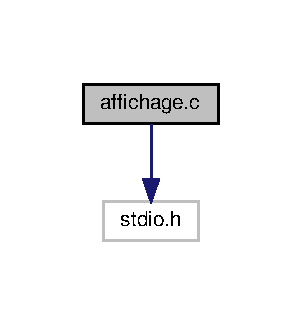
\includegraphics[width=145pt]{affichage_8c__incl}
\end{center}
\end{figure}
\subsection*{Functions}
\begin{DoxyCompactItemize}
\item 
\hyperlink{affichage_8c_abebc96b5336bc623acb55b3ef449e09a}{affiche\+Score} (int \mbox{[}$\,$\mbox{]} joueur) int \hyperlink{yahtzee_8c_ae66f6b31b5ad750f1fe042a706a4e3d4}{main}(int argc
\end{DoxyCompactItemize}
\subsection*{Variables}
\begin{DoxyCompactItemize}
\item 
char const  $\ast$ \hyperlink{affichage_8c_a6e043f967ef585fb48889d29b027b9bc}{argv} \mbox{[}$\,$\mbox{]}
\end{DoxyCompactItemize}


\subsection{Function Documentation}
\mbox{\Hypertarget{affichage_8c_abebc96b5336bc623acb55b3ef449e09a}\label{affichage_8c_abebc96b5336bc623acb55b3ef449e09a}} 
\index{affichage.\+c@{affichage.\+c}!affiche\+Score@{affiche\+Score}}
\index{affiche\+Score@{affiche\+Score}!affichage.\+c@{affichage.\+c}}
\subsubsection{\texorpdfstring{affiche\+Score()}{afficheScore()}}
{\footnotesize\ttfamily affiche\+Score (\begin{DoxyParamCaption}\item[{int \mbox{[}$\,$\mbox{]}}]{joueur }\end{DoxyParamCaption})}



\subsection{Variable Documentation}
\mbox{\Hypertarget{affichage_8c_a6e043f967ef585fb48889d29b027b9bc}\label{affichage_8c_a6e043f967ef585fb48889d29b027b9bc}} 
\index{affichage.\+c@{affichage.\+c}!argv@{argv}}
\index{argv@{argv}!affichage.\+c@{affichage.\+c}}
\subsubsection{\texorpdfstring{argv}{argv}}
{\footnotesize\ttfamily char const$\ast$ argv\mbox{[}$\,$\mbox{]}}

{\bfseries Initial value\+:}
\begin{DoxyCode}
\{
    
    \textcolor{keywordflow}{return} 0
\end{DoxyCode}


Definition at line 9 of file affichage.\+c.


\hypertarget{header_8h}{}\section{header.\+h File Reference}
\label{header_8h}\index{header.\+h@{header.\+h}}

\hypertarget{main_8c}{}\section{main.\+c File Reference}
\label{main_8c}\index{main.\+c@{main.\+c}}
{\ttfamily \#include \char`\"{}mecanisme\+Jeu.\+h\char`\"{}}\newline
{\ttfamily \#include $<$assert.\+h$>$}\newline
Include dependency graph for main.\+c\+:
\nopagebreak
\begin{figure}[H]
\begin{center}
\leavevmode
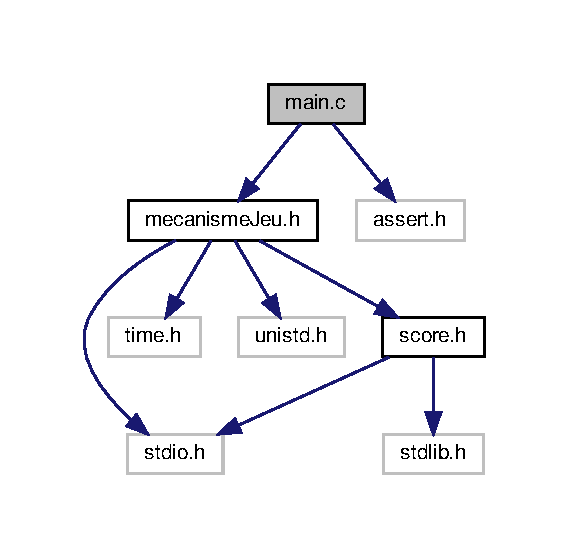
\includegraphics[width=273pt]{main_8c__incl}
\end{center}
\end{figure}
\subsection*{Macros}
\begin{DoxyCompactItemize}
\item 
\#define \hyperlink{main_8c_a4e9afb5e609dc54a28608e950d481fb1}{M\+A\+X\+\_\+\+P\+L\+A\+Y\+ER}~2
\end{DoxyCompactItemize}
\subsection*{Functions}
\begin{DoxyCompactItemize}
\item 
int \hyperlink{main_8c_ae66f6b31b5ad750f1fe042a706a4e3d4}{main} ()
\end{DoxyCompactItemize}


\subsection{Macro Definition Documentation}
\mbox{\Hypertarget{main_8c_a4e9afb5e609dc54a28608e950d481fb1}\label{main_8c_a4e9afb5e609dc54a28608e950d481fb1}} 
\index{main.\+c@{main.\+c}!M\+A\+X\+\_\+\+P\+L\+A\+Y\+ER@{M\+A\+X\+\_\+\+P\+L\+A\+Y\+ER}}
\index{M\+A\+X\+\_\+\+P\+L\+A\+Y\+ER@{M\+A\+X\+\_\+\+P\+L\+A\+Y\+ER}!main.\+c@{main.\+c}}
\subsubsection{\texorpdfstring{M\+A\+X\+\_\+\+P\+L\+A\+Y\+ER}{MAX\_PLAYER}}
{\footnotesize\ttfamily \#define M\+A\+X\+\_\+\+P\+L\+A\+Y\+ER~2}



Definition at line 3 of file main.\+c.



\subsection{Function Documentation}
\mbox{\Hypertarget{main_8c_ae66f6b31b5ad750f1fe042a706a4e3d4}\label{main_8c_ae66f6b31b5ad750f1fe042a706a4e3d4}} 
\index{main.\+c@{main.\+c}!main@{main}}
\index{main@{main}!main.\+c@{main.\+c}}
\subsubsection{\texorpdfstring{main()}{main()}}
{\footnotesize\ttfamily int main (\begin{DoxyParamCaption}{ }\end{DoxyParamCaption})}

Boucle main qui lance le jeu

Definition at line 5 of file main.\+c.



References compare\+Score(), complete\+Turn(), Player\+::dices, Player\+::dices\+Allowed, free\+Player(), M\+A\+X\+\_\+\+C\+O\+M\+B\+I\+N\+A\+T\+O\+I\+RE, Player\+::nbr\+Roll\+Remain, Player\+::score\+Final, Player\+::tab\+Score, and Player\+::tab\+Score\+Final.


\begin{DoxyCode}
6 \{
10     \hyperlink{structPlayer}{Player} *player1;
11     player1 = malloc(\textcolor{keyword}{sizeof} (\hyperlink{structPlayer}{Player}));
12     player1->\hyperlink{structPlayer_a676bd9687aaa50806f419c4ae170bcb2}{dices} = malloc(\textcolor{keyword}{sizeof}(\textcolor{keywordtype}{int})*7);
13     player1->\hyperlink{structPlayer_adb33524b9364f3e0bcfc5bd098cdaaf0}{dicesAllowed} = malloc(\textcolor{keyword}{sizeof}(\textcolor{keywordtype}{int})*7);
14     player1->\hyperlink{structPlayer_ae4c871b61a2af583a8b5975d736bea5d}{nbrRollRemain} = 6 ;
15     player1->\hyperlink{structPlayer_a7d5c0f37c78c868e4721cc8ceece92a6}{tabScore} = malloc(\textcolor{keyword}{sizeof}(\textcolor{keywordtype}{int})* \hyperlink{mecanismeJeu_8h_ac4569f5d2f9012ccdd6e3d25e9dbf7c5}{MAX\_COMBINATOIRE});
16     player1->\hyperlink{structPlayer_a7c377df37ea43f041207fc4de5ac0a93}{tabScoreFinal} = malloc(\textcolor{keyword}{sizeof}(\textcolor{keywordtype}{int})* \hyperlink{mecanismeJeu_8h_ac4569f5d2f9012ccdd6e3d25e9dbf7c5}{MAX\_COMBINATOIRE});
17     assert(player1->\hyperlink{structPlayer_a676bd9687aaa50806f419c4ae170bcb2}{dices});
18     assert(player1->\hyperlink{structPlayer_adb33524b9364f3e0bcfc5bd098cdaaf0}{dicesAllowed});
19     assert(player1->\hyperlink{structPlayer_a7d5c0f37c78c868e4721cc8ceece92a6}{tabScore});
20     assert(player1->\hyperlink{structPlayer_a7c377df37ea43f041207fc4de5ac0a93}{tabScoreFinal});
21 
22     \hyperlink{structPlayer}{Player} *player2;
23     player2 = malloc(\textcolor{keyword}{sizeof} (\hyperlink{structPlayer}{Player}));
24     player2->\hyperlink{structPlayer_a676bd9687aaa50806f419c4ae170bcb2}{dices} = malloc(\textcolor{keyword}{sizeof}(\textcolor{keywordtype}{int})*7);
25     player2->\hyperlink{structPlayer_adb33524b9364f3e0bcfc5bd098cdaaf0}{dicesAllowed} = malloc(\textcolor{keyword}{sizeof}(\textcolor{keywordtype}{int})*7);
26     player2->\hyperlink{structPlayer_ae4c871b61a2af583a8b5975d736bea5d}{nbrRollRemain} = 6 ;
27     player2->\hyperlink{structPlayer_a7d5c0f37c78c868e4721cc8ceece92a6}{tabScore} = malloc(\textcolor{keyword}{sizeof}(\textcolor{keywordtype}{int}*)* \hyperlink{mecanismeJeu_8h_ac4569f5d2f9012ccdd6e3d25e9dbf7c5}{MAX\_COMBINATOIRE});
28     player2->\hyperlink{structPlayer_a7c377df37ea43f041207fc4de5ac0a93}{tabScoreFinal} = malloc(\textcolor{keyword}{sizeof}(\textcolor{keywordtype}{int}*)* \hyperlink{mecanismeJeu_8h_ac4569f5d2f9012ccdd6e3d25e9dbf7c5}{MAX\_COMBINATOIRE});
29     assert(player2->\hyperlink{structPlayer_a676bd9687aaa50806f419c4ae170bcb2}{dices});
30     assert(player2->\hyperlink{structPlayer_adb33524b9364f3e0bcfc5bd098cdaaf0}{dicesAllowed});
31     assert(player2->\hyperlink{structPlayer_a7d5c0f37c78c868e4721cc8ceece92a6}{tabScore});
32     assert(player2->\hyperlink{structPlayer_a7c377df37ea43f041207fc4de5ac0a93}{tabScoreFinal});
33         
34     \textcolor{keywordflow}{for} (\textcolor{keywordtype}{int} i = 0; i < \hyperlink{mecanismeJeu_8h_ac4569f5d2f9012ccdd6e3d25e9dbf7c5}{MAX\_COMBINATOIRE}; ++i)
35     \{
36         player1->\hyperlink{structPlayer_a7d5c0f37c78c868e4721cc8ceece92a6}{tabScore}[i]= 0;
37         player1->\hyperlink{structPlayer_a7c377df37ea43f041207fc4de5ac0a93}{tabScoreFinal}[i]=-1;
38         player2->\hyperlink{structPlayer_a7d5c0f37c78c868e4721cc8ceece92a6}{tabScore}[i]= 0;
39         player2->\hyperlink{structPlayer_a7c377df37ea43f041207fc4de5ac0a93}{tabScoreFinal}[i]=-1;
40     \}
41     
42     \textcolor{keywordtype}{int} nombreTour=12;
43 
44 
45 
46     \textcolor{keywordflow}{while} (nombreTour > 0)\{
47         printf(\textcolor{stringliteral}{"=============== C'est au Joueur %d de jouer ===============!\(\backslash\)n"}, 1);
48         \hyperlink{mecanismeJeu_8c_a9ccbcda936f74ce7cb8471cc41b8415e}{completeTurn}(player1);
49         printf(\textcolor{stringliteral}{"\(\backslash\)n\(\backslash\)n"});
50         printf(\textcolor{stringliteral}{"=============== C'est au Joueur %d de jouer ===============!\(\backslash\)n"}, 2);
51         
52         \hyperlink{mecanismeJeu_8c_a9ccbcda936f74ce7cb8471cc41b8415e}{completeTurn}(player2);
53         
54         --nombreTour;
55     \}
56     \hyperlink{score_8c_aeeb20f2b14b47a496fadd754abda5317}{compareScore}(player1->\hyperlink{structPlayer_a44cb6ebf8f95f9bd12f5985c9e5dfd99}{scoreFinal},player2->\hyperlink{structPlayer_a44cb6ebf8f95f9bd12f5985c9e5dfd99}{scoreFinal});
57 
58 \textcolor{comment}{//  fin des tours }
59     \textcolor{comment}{//>> felicite le gagant en affichant son score;}
60     
61     \hyperlink{mecanismeJeu_8c_afb996747437467dc9e569a34c469d31b}{freePlayer}(player1);
62     \hyperlink{mecanismeJeu_8c_afb996747437467dc9e569a34c469d31b}{freePlayer}(player2);
63 
64     \textcolor{keywordflow}{return} 0;
65 \}
\end{DoxyCode}
Here is the call graph for this function\+:
\nopagebreak
\begin{figure}[H]
\begin{center}
\leavevmode
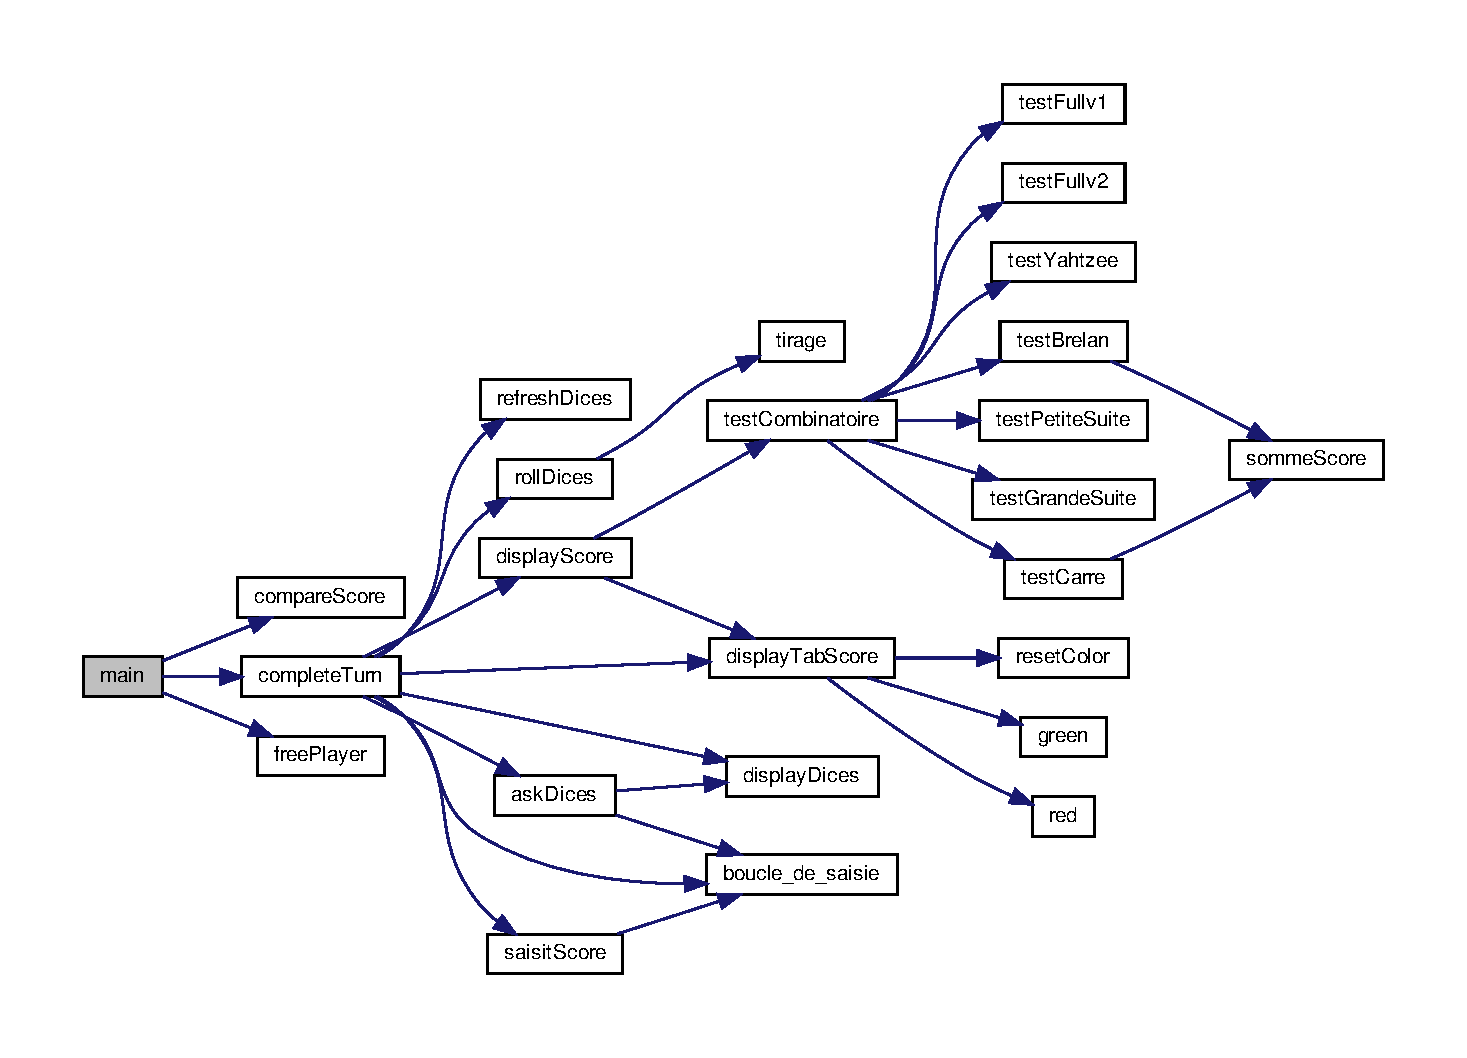
\includegraphics[width=350pt]{main_8c_ae66f6b31b5ad750f1fe042a706a4e3d4_cgraph}
\end{center}
\end{figure}

\hypertarget{mecanismeJeu_8c}{}\section{mecanisme\+Jeu.\+c File Reference}
\label{mecanismeJeu_8c}\index{mecanisme\+Jeu.\+c@{mecanisme\+Jeu.\+c}}
{\ttfamily \#include $<$stdio.\+h$>$}\newline
{\ttfamily \#include $<$stdlib.\+h$>$}\newline
{\ttfamily \#include \char`\"{}mecanisme\+Jeu.\+h\char`\"{}}\newline
{\ttfamily \#include \char`\"{}score.\+h\char`\"{}}\newline
Include dependency graph for mecanisme\+Jeu.\+c\+:
\nopagebreak
\begin{figure}[H]
\begin{center}
\leavevmode
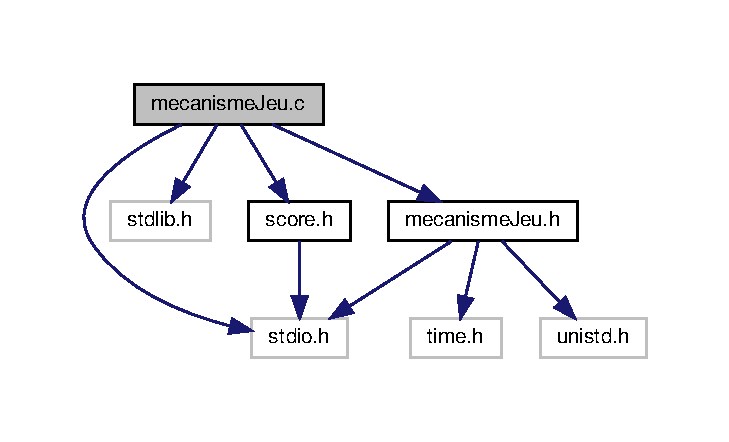
\includegraphics[width=350pt]{mecanismeJeu_8c__incl}
\end{center}
\end{figure}
\subsection*{Functions}
\begin{DoxyCompactItemize}
\item 
int \hyperlink{mecanismeJeu_8c_aedc55fd9756d84e32e3f03e04f964076}{tirage} (int max)
\item 
void \hyperlink{mecanismeJeu_8c_ab55e6b5866c616840bef8cccef4952c5}{roll\+Dices} (\hyperlink{structPlayer}{Player} $\ast$p)
\item 
void \hyperlink{mecanismeJeu_8c_acfee2b60324d906c1d4174e6e51b92d3}{refresh\+Dices} (\hyperlink{structPlayer}{Player} $\ast$p)
\item 
int \hyperlink{mecanismeJeu_8c_af34915129a343bf4c2718354a681f1fb}{boucle\+\_\+de\+\_\+saisie} (int a, int b)
\item 
void \hyperlink{mecanismeJeu_8c_ad9ebcce43b3be9b75d300f961d53d329}{display\+Dices} (\hyperlink{structPlayer}{Player} $\ast$p)
\item 
void \hyperlink{mecanismeJeu_8c_a9e4530f74b630f0cfcc27b8bddb34ce8}{ask\+Dices} (\hyperlink{structPlayer}{Player} $\ast$p)
\item 
void \hyperlink{mecanismeJeu_8c_a9ccbcda936f74ce7cb8471cc41b8415e}{complete\+Turn} (\hyperlink{structPlayer}{Player} $\ast$p)
\item 
void \hyperlink{mecanismeJeu_8c_afb996747437467dc9e569a34c469d31b}{free\+Player} (\hyperlink{structPlayer}{Player} $\ast$p)
\item 
void \hyperlink{mecanismeJeu_8c_a666fd7e17272b378e2cc99b811be39a5}{init\+Player} (\hyperlink{structPlayer}{Player} $\ast$p)
\end{DoxyCompactItemize}


\subsection{Function Documentation}
\mbox{\Hypertarget{mecanismeJeu_8c_a9e4530f74b630f0cfcc27b8bddb34ce8}\label{mecanismeJeu_8c_a9e4530f74b630f0cfcc27b8bddb34ce8}} 
\index{mecanisme\+Jeu.\+c@{mecanisme\+Jeu.\+c}!ask\+Dices@{ask\+Dices}}
\index{ask\+Dices@{ask\+Dices}!mecanisme\+Jeu.\+c@{mecanisme\+Jeu.\+c}}
\subsubsection{\texorpdfstring{ask\+Dices()}{askDices()}}
{\footnotesize\ttfamily void ask\+Dices (\begin{DoxyParamCaption}\item[{\hyperlink{structPlayer}{Player} $\ast$}]{p }\end{DoxyParamCaption})}



Definition at line 51 of file mecanisme\+Jeu.\+c.



References boucle\+\_\+de\+\_\+saisie().



Referenced by complete\+Turn().


\begin{DoxyCode}
51                         \{
52   \textcolor{keywordflow}{for} (\textcolor{keywordtype}{int} i = 0; i <8; ++i)
53   \{
54     \textcolor{keywordflow}{if}(p-> dicesAllowed[i]==1)\{
55       printf(\textcolor{stringliteral}{"voulez vous relancer le de %d ?\(\backslash\)n"},i+1 );
56       p-> dicesAllowed[i]= \hyperlink{mecanismeJeu_8c_af34915129a343bf4c2718354a681f1fb}{boucle\_de\_saisie}(0,1);
57     \} 
58   \}
59 
60 \}
\end{DoxyCode}
Here is the call graph for this function\+:
\nopagebreak
\begin{figure}[H]
\begin{center}
\leavevmode
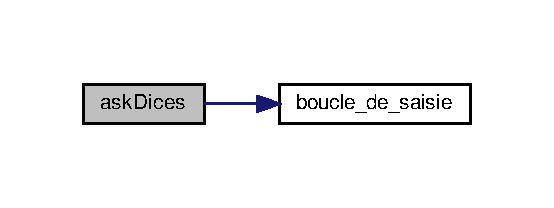
\includegraphics[width=266pt]{mecanismeJeu_8c_a9e4530f74b630f0cfcc27b8bddb34ce8_cgraph}
\end{center}
\end{figure}
Here is the caller graph for this function\+:
\nopagebreak
\begin{figure}[H]
\begin{center}
\leavevmode
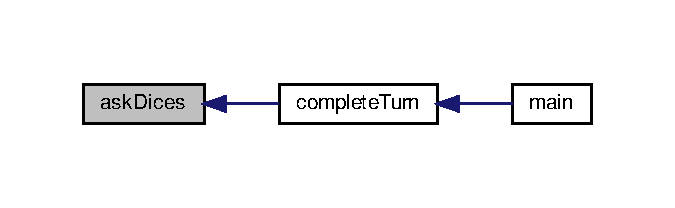
\includegraphics[width=324pt]{mecanismeJeu_8c_a9e4530f74b630f0cfcc27b8bddb34ce8_icgraph}
\end{center}
\end{figure}
\mbox{\Hypertarget{mecanismeJeu_8c_af34915129a343bf4c2718354a681f1fb}\label{mecanismeJeu_8c_af34915129a343bf4c2718354a681f1fb}} 
\index{mecanisme\+Jeu.\+c@{mecanisme\+Jeu.\+c}!boucle\+\_\+de\+\_\+saisie@{boucle\+\_\+de\+\_\+saisie}}
\index{boucle\+\_\+de\+\_\+saisie@{boucle\+\_\+de\+\_\+saisie}!mecanisme\+Jeu.\+c@{mecanisme\+Jeu.\+c}}
\subsubsection{\texorpdfstring{boucle\+\_\+de\+\_\+saisie()}{boucle\_de\_saisie()}}
{\footnotesize\ttfamily int boucle\+\_\+de\+\_\+saisie (\begin{DoxyParamCaption}\item[{int}]{a,  }\item[{int}]{b }\end{DoxyParamCaption})}



Definition at line 32 of file mecanisme\+Jeu.\+c.



Referenced by ask\+Dices(), and complete\+Turn().


\begin{DoxyCode}
32                                   \{
33     \textcolor{comment}{//retourne l'entier i ssi il est compris dans intervalle [a,b]}
34     \textcolor{keywordtype}{int} i;
35     \textcolor{keywordflow}{do}\{
36         fflush(stdin);
37         printf(\textcolor{stringliteral}{"merci de saisir un nombre compris entre %d et %d\(\backslash\)n"}, a, b);
38         scanf(\textcolor{stringliteral}{"%d"},&i);
39     \}\textcolor{keywordflow}{while}( i <a || i>b ||\textcolor{keyword}{sizeof}(i) != \textcolor{keyword}{sizeof}(\textcolor{keywordtype}{int}) );
40     \textcolor{keywordflow}{return} i;
41 \}
\end{DoxyCode}
Here is the caller graph for this function\+:
\nopagebreak
\begin{figure}[H]
\begin{center}
\leavevmode
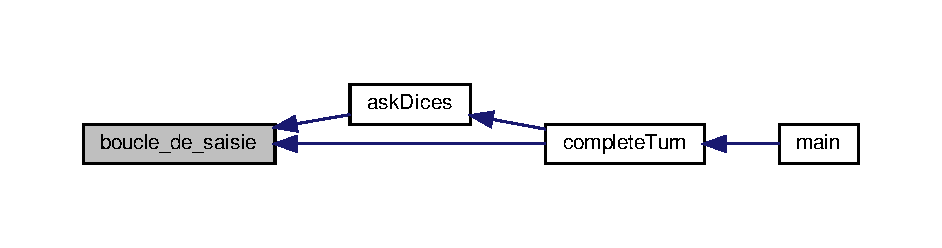
\includegraphics[width=350pt]{mecanismeJeu_8c_af34915129a343bf4c2718354a681f1fb_icgraph}
\end{center}
\end{figure}
\mbox{\Hypertarget{mecanismeJeu_8c_a9ccbcda936f74ce7cb8471cc41b8415e}\label{mecanismeJeu_8c_a9ccbcda936f74ce7cb8471cc41b8415e}} 
\index{mecanisme\+Jeu.\+c@{mecanisme\+Jeu.\+c}!complete\+Turn@{complete\+Turn}}
\index{complete\+Turn@{complete\+Turn}!mecanisme\+Jeu.\+c@{mecanisme\+Jeu.\+c}}
\subsubsection{\texorpdfstring{complete\+Turn()}{completeTurn()}}
{\footnotesize\ttfamily void complete\+Turn (\begin{DoxyParamCaption}\item[{\hyperlink{structPlayer}{Player} $\ast$}]{p }\end{DoxyParamCaption})}



Definition at line 63 of file mecanisme\+Jeu.\+c.



Referenced by main().


\begin{DoxyCode}
63                             \{
64   \textcolor{keywordtype}{int} v = 1 ;
65   \hyperlink{mecanismeJeu_8c_acfee2b60324d906c1d4174e6e51b92d3}{refreshDices}(p) ;
66   \hyperlink{mecanismeJeu_8c_ab55e6b5866c616840bef8cccef4952c5}{rollDices}(p) ;   
67 
68   p->\hyperlink{structPlayer_ae4c871b61a2af583a8b5975d736bea5d}{nbrRollRemain} -= 1 ;
69   \textcolor{keywordflow}{while}(p->\hyperlink{structPlayer_ae4c871b61a2af583a8b5975d736bea5d}{nbrRollRemain} != 0)\{
70     printf(\textcolor{stringliteral}{"Lancé de dée :\(\backslash\)n"}) ;
71     \hyperlink{mecanismeJeu_8c_ad9ebcce43b3be9b75d300f961d53d329}{displayDices}(p) ;
72     printf(\textcolor{stringliteral}{"Voulez vous relancer des dées ? "}) ;
73     v = \hyperlink{mecanismeJeu_8c_af34915129a343bf4c2718354a681f1fb}{boucle\_de\_saisie}(0,1) ;
74     \textcolor{keywordflow}{if}(v == 0) \{ \textcolor{comment}{// cas fin de lance}
75       p->\hyperlink{structPlayer_ae4c871b61a2af583a8b5975d736bea5d}{nbrRollRemain} = 0 ; 
76       \hyperlink{score_8c_a54d088aca7937ae9e67dabbe160f5254}{displayScore}(p->\hyperlink{structPlayer_a7d5c0f37c78c868e4721cc8ceece92a6}{tabScore},p->\hyperlink{structPlayer_a676bd9687aaa50806f419c4ae170bcb2}{dices});
77       \} 
78     
79 
80     \textcolor{keywordflow}{else}\{ \textcolor{comment}{//cas relance de}
81       \textcolor{keywordflow}{if}(p->\hyperlink{structPlayer_ae4c871b61a2af583a8b5975d736bea5d}{nbrRollRemain} !=6)printf(\textcolor{stringliteral}{"lequelles one ? "}) ;
82       \hyperlink{mecanismeJeu_8c_a9e4530f74b630f0cfcc27b8bddb34ce8}{askDices}(p);
83       p->\hyperlink{structPlayer_ae4c871b61a2af583a8b5975d736bea5d}{nbrRollRemain} -= 1 ;
84       \hyperlink{mecanismeJeu_8c_ab55e6b5866c616840bef8cccef4952c5}{rollDices}(p) ;
85       printf(\textcolor{stringliteral}{"Vous avez relancé des dées :\(\backslash\)n"}) ;
86       \hyperlink{score_8c_a54d088aca7937ae9e67dabbe160f5254}{displayScore}(p->\hyperlink{structPlayer_a7d5c0f37c78c868e4721cc8ceece92a6}{tabScore},p->\hyperlink{structPlayer_a676bd9687aaa50806f419c4ae170bcb2}{dices});
87       printf(\textcolor{stringliteral}{"Essaies restante : %d\(\backslash\)n"}, p->\hyperlink{structPlayer_ae4c871b61a2af583a8b5975d736bea5d}{nbrRollRemain}) ; 
88     \}
89   \}
90   printf(\textcolor{stringliteral}{"Tour du prochain joueur\(\backslash\)n"}) ;
91 \}
\end{DoxyCode}
Here is the caller graph for this function\+:
\nopagebreak
\begin{figure}[H]
\begin{center}
\leavevmode
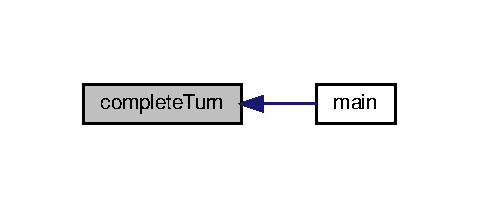
\includegraphics[width=230pt]{mecanismeJeu_8c_a9ccbcda936f74ce7cb8471cc41b8415e_icgraph}
\end{center}
\end{figure}
\mbox{\Hypertarget{mecanismeJeu_8c_ad9ebcce43b3be9b75d300f961d53d329}\label{mecanismeJeu_8c_ad9ebcce43b3be9b75d300f961d53d329}} 
\index{mecanisme\+Jeu.\+c@{mecanisme\+Jeu.\+c}!display\+Dices@{display\+Dices}}
\index{display\+Dices@{display\+Dices}!mecanisme\+Jeu.\+c@{mecanisme\+Jeu.\+c}}
\subsubsection{\texorpdfstring{display\+Dices()}{displayDices()}}
{\footnotesize\ttfamily void display\+Dices (\begin{DoxyParamCaption}\item[{\hyperlink{structPlayer}{Player} $\ast$}]{p }\end{DoxyParamCaption})}



Definition at line 43 of file mecanisme\+Jeu.\+c.



References Player\+::dices.



Referenced by complete\+Turn().


\begin{DoxyCode}
43                             \{
44   \textcolor{keywordflow}{for}(\textcolor{keywordtype}{int} i = 0 ; i < 8 ; ++i)\{
45     printf(\textcolor{stringliteral}{"%d "}, p->\hyperlink{structPlayer_a676bd9687aaa50806f419c4ae170bcb2}{dices}[i]) ;
46   \}
47   
48   printf(\textcolor{stringliteral}{"\(\backslash\)n"}) ;
49 \}
\end{DoxyCode}
Here is the caller graph for this function\+:
\nopagebreak
\begin{figure}[H]
\begin{center}
\leavevmode
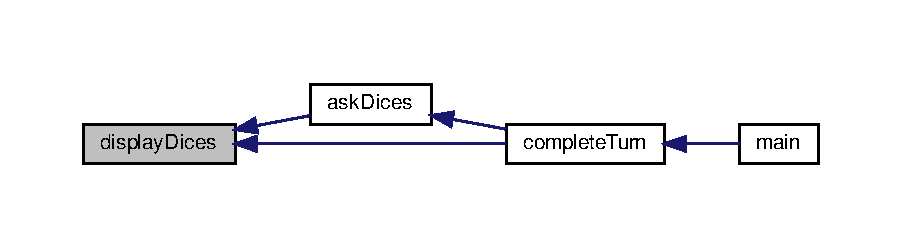
\includegraphics[width=339pt]{mecanismeJeu_8c_ad9ebcce43b3be9b75d300f961d53d329_icgraph}
\end{center}
\end{figure}
\mbox{\Hypertarget{mecanismeJeu_8c_afb996747437467dc9e569a34c469d31b}\label{mecanismeJeu_8c_afb996747437467dc9e569a34c469d31b}} 
\index{mecanisme\+Jeu.\+c@{mecanisme\+Jeu.\+c}!free\+Player@{free\+Player}}
\index{free\+Player@{free\+Player}!mecanisme\+Jeu.\+c@{mecanisme\+Jeu.\+c}}
\subsubsection{\texorpdfstring{free\+Player()}{freePlayer()}}
{\footnotesize\ttfamily void free\+Player (\begin{DoxyParamCaption}\item[{\hyperlink{structPlayer}{Player} $\ast$}]{p }\end{DoxyParamCaption})}



Definition at line 93 of file mecanisme\+Jeu.\+c.



References Player\+::dices, Player\+::dices\+Allowed, and Player\+::tab\+Score.



Referenced by main().


\begin{DoxyCode}
93                           \{
94   free(p->\hyperlink{structPlayer_a676bd9687aaa50806f419c4ae170bcb2}{dices});
95   free(p->\hyperlink{structPlayer_adb33524b9364f3e0bcfc5bd098cdaaf0}{dicesAllowed});
96   free(p->\hyperlink{structPlayer_a7d5c0f37c78c868e4721cc8ceece92a6}{tabScore});
97 \}
\end{DoxyCode}
Here is the caller graph for this function\+:
\nopagebreak
\begin{figure}[H]
\begin{center}
\leavevmode
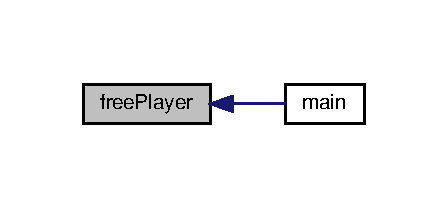
\includegraphics[width=215pt]{mecanismeJeu_8c_afb996747437467dc9e569a34c469d31b_icgraph}
\end{center}
\end{figure}
\mbox{\Hypertarget{mecanismeJeu_8c_a666fd7e17272b378e2cc99b811be39a5}\label{mecanismeJeu_8c_a666fd7e17272b378e2cc99b811be39a5}} 
\index{mecanisme\+Jeu.\+c@{mecanisme\+Jeu.\+c}!init\+Player@{init\+Player}}
\index{init\+Player@{init\+Player}!mecanisme\+Jeu.\+c@{mecanisme\+Jeu.\+c}}
\subsubsection{\texorpdfstring{init\+Player()}{initPlayer()}}
{\footnotesize\ttfamily void init\+Player (\begin{DoxyParamCaption}\item[{\hyperlink{structPlayer}{Player} $\ast$}]{p }\end{DoxyParamCaption})}



Definition at line 98 of file mecanisme\+Jeu.\+c.



References Player\+::dices, Player\+::dices\+Allowed, Player\+::nbr\+Roll\+Remain, Player\+::score, and Player\+::tab\+Score.



Referenced by main().


\begin{DoxyCode}
98                           \{
99   \textcolor{comment}{//askName();}
100   p->\hyperlink{structPlayer_a676bd9687aaa50806f419c4ae170bcb2}{dices} = malloc(\textcolor{keyword}{sizeof}(\textcolor{keywordtype}{int})*8);
101   p->\hyperlink{structPlayer_adb33524b9364f3e0bcfc5bd098cdaaf0}{dicesAllowed} = malloc(\textcolor{keyword}{sizeof}(\textcolor{keywordtype}{int})*8);
102   p->\hyperlink{structPlayer_ae4c871b61a2af583a8b5975d736bea5d}{nbrRollRemain} = 6 ;
103   p->\hyperlink{structPlayer_ace6abae8d66534ad0a1fd6458f786a6e}{score} = 0;
104   p->\hyperlink{structPlayer_a7d5c0f37c78c868e4721cc8ceece92a6}{tabScore} = malloc(\textcolor{keyword}{sizeof}(\textcolor{keywordtype}{int})*6);
105   \textcolor{keywordflow}{for} (\textcolor{keywordtype}{int} i = 0; i < 6; ++i)
106   \{
107     p->\hyperlink{structPlayer_a7d5c0f37c78c868e4721cc8ceece92a6}{tabScore}[i]= 0;
108   \}
109 \}
\end{DoxyCode}
Here is the caller graph for this function\+:
\nopagebreak
\begin{figure}[H]
\begin{center}
\leavevmode
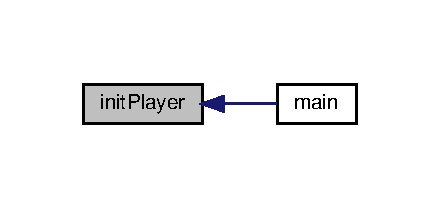
\includegraphics[width=211pt]{mecanismeJeu_8c_a666fd7e17272b378e2cc99b811be39a5_icgraph}
\end{center}
\end{figure}
\mbox{\Hypertarget{mecanismeJeu_8c_acfee2b60324d906c1d4174e6e51b92d3}\label{mecanismeJeu_8c_acfee2b60324d906c1d4174e6e51b92d3}} 
\index{mecanisme\+Jeu.\+c@{mecanisme\+Jeu.\+c}!refresh\+Dices@{refresh\+Dices}}
\index{refresh\+Dices@{refresh\+Dices}!mecanisme\+Jeu.\+c@{mecanisme\+Jeu.\+c}}
\subsubsection{\texorpdfstring{refresh\+Dices()}{refreshDices()}}
{\footnotesize\ttfamily void refresh\+Dices (\begin{DoxyParamCaption}\item[{\hyperlink{structPlayer}{Player} $\ast$}]{p }\end{DoxyParamCaption})}



Definition at line 23 of file mecanisme\+Jeu.\+c.



References Player\+::dices, and Player\+::dices\+Allowed.



Referenced by complete\+Turn().


\begin{DoxyCode}
23                             \{
24 
25   \textcolor{keywordflow}{for}(\textcolor{keywordtype}{int} i = 0 ; i < 8 ; ++i)\{
26     p->\hyperlink{structPlayer_a676bd9687aaa50806f419c4ae170bcb2}{dices}[i] = 0 ;
27     p->\hyperlink{structPlayer_adb33524b9364f3e0bcfc5bd098cdaaf0}{dicesAllowed}[i]=1;
28   \} 
29 \}
\end{DoxyCode}
Here is the caller graph for this function\+:
\nopagebreak
\begin{figure}[H]
\begin{center}
\leavevmode
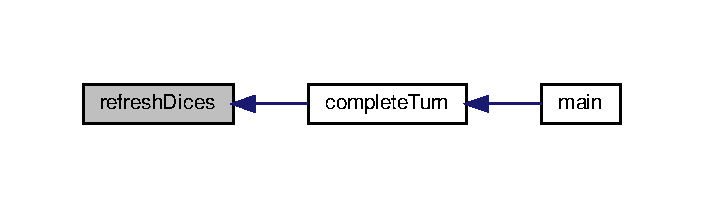
\includegraphics[width=338pt]{mecanismeJeu_8c_acfee2b60324d906c1d4174e6e51b92d3_icgraph}
\end{center}
\end{figure}
\mbox{\Hypertarget{mecanismeJeu_8c_ab55e6b5866c616840bef8cccef4952c5}\label{mecanismeJeu_8c_ab55e6b5866c616840bef8cccef4952c5}} 
\index{mecanisme\+Jeu.\+c@{mecanisme\+Jeu.\+c}!roll\+Dices@{roll\+Dices}}
\index{roll\+Dices@{roll\+Dices}!mecanisme\+Jeu.\+c@{mecanisme\+Jeu.\+c}}
\subsubsection{\texorpdfstring{roll\+Dices()}{rollDices()}}
{\footnotesize\ttfamily void roll\+Dices (\begin{DoxyParamCaption}\item[{\hyperlink{structPlayer}{Player} $\ast$}]{p }\end{DoxyParamCaption})}



Definition at line 13 of file mecanisme\+Jeu.\+c.



References Player\+::dices, Player\+::dices\+Allowed, and tirage().



Referenced by complete\+Turn().


\begin{DoxyCode}
13                          \{
14   srand((\textcolor{keywordtype}{unsigned})time(NULL));\textcolor{comment}{//set Seed pour le tirage}
15   \textcolor{keywordflow}{for}(\textcolor{keywordtype}{int} i = 0 ; i < 8; ++i)\{
16     \textcolor{keywordflow}{if} (p->\hyperlink{structPlayer_adb33524b9364f3e0bcfc5bd098cdaaf0}{dicesAllowed}[i])\{
17       p->\hyperlink{structPlayer_a676bd9687aaa50806f419c4ae170bcb2}{dices}[i] = \hyperlink{mecanismeJeu_8c_aedc55fd9756d84e32e3f03e04f964076}{tirage}(8) ;
18       \textcolor{comment}{//printf(">>>de %d tire%d\(\backslash\)n",i,p->dices[i] );}
19     \}
20   \}
21 \}
\end{DoxyCode}
Here is the call graph for this function\+:
\nopagebreak
\begin{figure}[H]
\begin{center}
\leavevmode
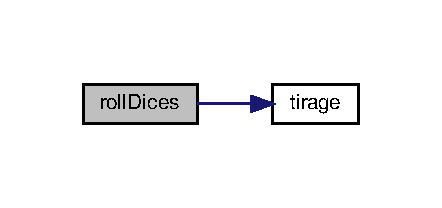
\includegraphics[width=212pt]{mecanismeJeu_8c_ab55e6b5866c616840bef8cccef4952c5_cgraph}
\end{center}
\end{figure}
Here is the caller graph for this function\+:
\nopagebreak
\begin{figure}[H]
\begin{center}
\leavevmode
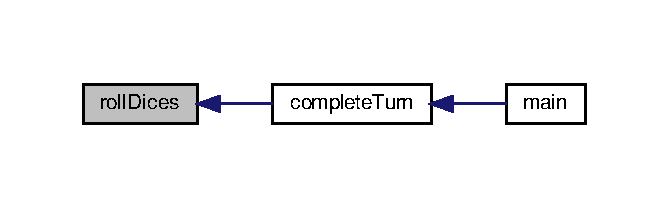
\includegraphics[width=321pt]{mecanismeJeu_8c_ab55e6b5866c616840bef8cccef4952c5_icgraph}
\end{center}
\end{figure}
\mbox{\Hypertarget{mecanismeJeu_8c_aedc55fd9756d84e32e3f03e04f964076}\label{mecanismeJeu_8c_aedc55fd9756d84e32e3f03e04f964076}} 
\index{mecanisme\+Jeu.\+c@{mecanisme\+Jeu.\+c}!tirage@{tirage}}
\index{tirage@{tirage}!mecanisme\+Jeu.\+c@{mecanisme\+Jeu.\+c}}
\subsubsection{\texorpdfstring{tirage()}{tirage()}}
{\footnotesize\ttfamily int tirage (\begin{DoxyParamCaption}\item[{int}]{max }\end{DoxyParamCaption})}



Definition at line 6 of file mecanisme\+Jeu.\+c.



Referenced by roll\+Dices().


\begin{DoxyCode}
6                    \{
7     \textcolor{comment}{/*tire au sort un nombre compris entre 0 inclus max; }
8 \textcolor{comment}{    srand((unsigned)time(NULL));*/}
9     rand();
10     \textcolor{keywordflow}{return} (\textcolor{keywordtype}{double})(rand()/(double)(RAND\_MAX) * (max))+1;
11 \}
\end{DoxyCode}
Here is the caller graph for this function\+:
\nopagebreak
\begin{figure}[H]
\begin{center}
\leavevmode
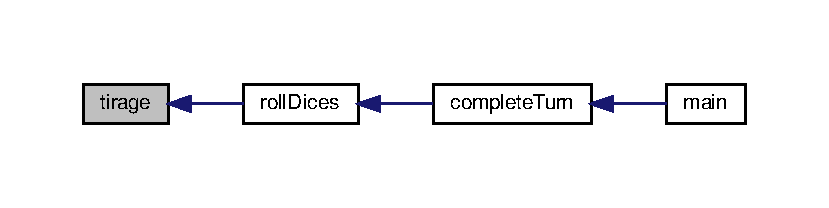
\includegraphics[width=350pt]{mecanismeJeu_8c_aedc55fd9756d84e32e3f03e04f964076_icgraph}
\end{center}
\end{figure}

\hypertarget{mecanismeJeu_8h}{}\section{mecanisme\+Jeu.\+h File Reference}
\label{mecanismeJeu_8h}\index{mecanisme\+Jeu.\+h@{mecanisme\+Jeu.\+h}}
{\ttfamily \#include $<$stdio.\+h$>$}\newline
{\ttfamily \#include $<$time.\+h$>$}\newline
{\ttfamily \#include $<$unistd.\+h$>$}\newline
{\ttfamily \#include \char`\"{}score.\+h\char`\"{}}\newline
Include dependency graph for mecanisme\+Jeu.\+h\+:
\nopagebreak
\begin{figure}[H]
\begin{center}
\leavevmode
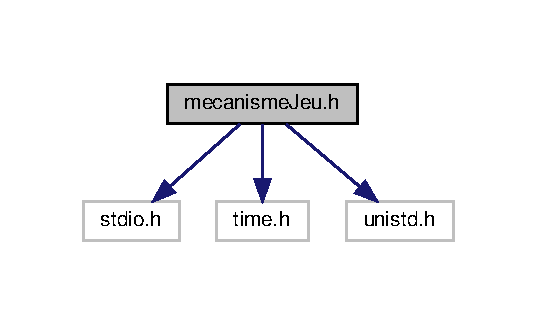
\includegraphics[width=273pt]{mecanismeJeu_8h__incl}
\end{center}
\end{figure}
This graph shows which files directly or indirectly include this file\+:
\nopagebreak
\begin{figure}[H]
\begin{center}
\leavevmode
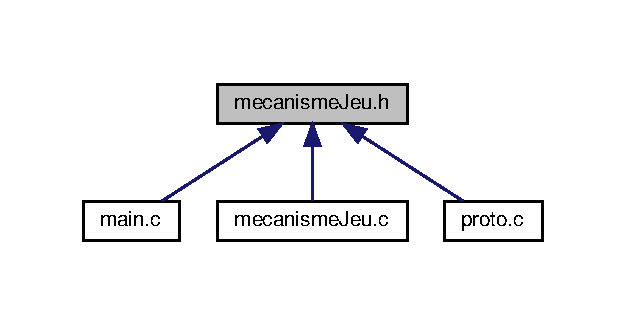
\includegraphics[width=236pt]{mecanismeJeu_8h__dep__incl}
\end{center}
\end{figure}
\subsection*{Data Structures}
\begin{DoxyCompactItemize}
\item 
struct \hyperlink{structPlayer}{Player}
\end{DoxyCompactItemize}
\subsection*{Macros}
\begin{DoxyCompactItemize}
\item 
\#define \hyperlink{mecanismeJeu_8h_ac4569f5d2f9012ccdd6e3d25e9dbf7c5}{M\+A\+X\+\_\+\+C\+O\+M\+B\+I\+N\+A\+T\+O\+I\+RE}~20
\end{DoxyCompactItemize}
\subsection*{Typedefs}
\begin{DoxyCompactItemize}
\item 
typedef struct \hyperlink{structPlayer}{Player} \hyperlink{mecanismeJeu_8h_a480a040facb94f90060562cd65274385}{Player}
\end{DoxyCompactItemize}
\subsection*{Functions}
\begin{DoxyCompactItemize}
\item 
int \hyperlink{mecanismeJeu_8h_aedc55fd9756d84e32e3f03e04f964076}{tirage} (int max)
\begin{DoxyCompactList}\small\item\em donne la valeur de dée \end{DoxyCompactList}\item 
void \hyperlink{mecanismeJeu_8h_ab55e6b5866c616840bef8cccef4952c5}{roll\+Dices} (\hyperlink{structPlayer}{Player} $\ast$p)
\begin{DoxyCompactList}\small\item\em la coup de jeu \end{DoxyCompactList}\item 
void \hyperlink{mecanismeJeu_8h_acfee2b60324d906c1d4174e6e51b92d3}{refresh\+Dices} (\hyperlink{structPlayer}{Player} $\ast$p)
\begin{DoxyCompactList}\small\item\em initialise les dées \end{DoxyCompactList}\item 
void \hyperlink{mecanismeJeu_8h_ad9ebcce43b3be9b75d300f961d53d329}{display\+Dices} (\hyperlink{structPlayer}{Player} $\ast$p)
\begin{DoxyCompactList}\small\item\em affichage des dées. \end{DoxyCompactList}\item 
void \hyperlink{mecanismeJeu_8h_a9e4530f74b630f0cfcc27b8bddb34ce8}{ask\+Dices} (\hyperlink{structPlayer}{Player} $\ast$p)
\begin{DoxyCompactList}\small\item\em relance les dées \end{DoxyCompactList}\item 
void \hyperlink{mecanismeJeu_8h_a9ccbcda936f74ce7cb8471cc41b8415e}{complete\+Turn} (\hyperlink{structPlayer}{Player} $\ast$p)
\begin{DoxyCompactList}\small\item\em lance une partie de jeu. \end{DoxyCompactList}\item 
void \hyperlink{mecanismeJeu_8h_afb996747437467dc9e569a34c469d31b}{free\+Player} (\hyperlink{structPlayer}{Player} $\ast$p)
\begin{DoxyCompactList}\small\item\em libére la memoire. \end{DoxyCompactList}\end{DoxyCompactItemize}


\subsection{Macro Definition Documentation}
\mbox{\Hypertarget{mecanismeJeu_8h_ac4569f5d2f9012ccdd6e3d25e9dbf7c5}\label{mecanismeJeu_8h_ac4569f5d2f9012ccdd6e3d25e9dbf7c5}} 
\index{mecanisme\+Jeu.\+h@{mecanisme\+Jeu.\+h}!M\+A\+X\+\_\+\+C\+O\+M\+B\+I\+N\+A\+T\+O\+I\+RE@{M\+A\+X\+\_\+\+C\+O\+M\+B\+I\+N\+A\+T\+O\+I\+RE}}
\index{M\+A\+X\+\_\+\+C\+O\+M\+B\+I\+N\+A\+T\+O\+I\+RE@{M\+A\+X\+\_\+\+C\+O\+M\+B\+I\+N\+A\+T\+O\+I\+RE}!mecanisme\+Jeu.\+h@{mecanisme\+Jeu.\+h}}
\subsubsection{\texorpdfstring{M\+A\+X\+\_\+\+C\+O\+M\+B\+I\+N\+A\+T\+O\+I\+RE}{MAX\_COMBINATOIRE}}
{\footnotesize\ttfamily \#define M\+A\+X\+\_\+\+C\+O\+M\+B\+I\+N\+A\+T\+O\+I\+RE~20}



Definition at line 5 of file mecanisme\+Jeu.\+h.



Referenced by main().



\subsection{Typedef Documentation}
\mbox{\Hypertarget{mecanismeJeu_8h_a480a040facb94f90060562cd65274385}\label{mecanismeJeu_8h_a480a040facb94f90060562cd65274385}} 
\index{mecanisme\+Jeu.\+h@{mecanisme\+Jeu.\+h}!Player@{Player}}
\index{Player@{Player}!mecanisme\+Jeu.\+h@{mecanisme\+Jeu.\+h}}
\subsubsection{\texorpdfstring{Player}{Player}}
{\footnotesize\ttfamily typedef struct \hyperlink{structPlayer}{Player} \hyperlink{structPlayer}{Player}}



Definition at line 8 of file mecanisme\+Jeu.\+h.



\subsection{Function Documentation}
\mbox{\Hypertarget{mecanismeJeu_8h_a9e4530f74b630f0cfcc27b8bddb34ce8}\label{mecanismeJeu_8h_a9e4530f74b630f0cfcc27b8bddb34ce8}} 
\index{mecanisme\+Jeu.\+h@{mecanisme\+Jeu.\+h}!ask\+Dices@{ask\+Dices}}
\index{ask\+Dices@{ask\+Dices}!mecanisme\+Jeu.\+h@{mecanisme\+Jeu.\+h}}
\subsubsection{\texorpdfstring{ask\+Dices()}{askDices()}}
{\footnotesize\ttfamily void ask\+Dices (\begin{DoxyParamCaption}\item[{\hyperlink{structPlayer}{Player} $\ast$}]{p }\end{DoxyParamCaption})}



relance les dées 

demande au joueur s\textquotesingle{}il veurt relancer le dée. 
\begin{DoxyParams}{Parameters}
{\em p} & le joueur. \\
\hline
\end{DoxyParams}


Definition at line 76 of file mecanisme\+Jeu.\+c.



References boucle\+\_\+de\+\_\+saisie(), Player\+::dices, Player\+::dices\+Allowed, and display\+Dices().



Referenced by complete\+Turn().


\begin{DoxyCode}
76                         \{
77   \textcolor{keywordflow}{for} (\textcolor{keywordtype}{int} i = 0; i <7; ++i)
78   \{\hyperlink{mecanismeJeu_8c_ad9ebcce43b3be9b75d300f961d53d329}{displayDices}(p);
79     \textcolor{keywordflow}{if}(p-> dicesAllowed[i]==1)\{
80       
81       printf(\textcolor{stringliteral}{"voulez vous relancer le de %d ?\(\backslash\)n"},p->\hyperlink{structPlayer_a676bd9687aaa50806f419c4ae170bcb2}{dices}[i] );
82       \hyperlink{score_8c_a1e229810418844ae6a50ff60d258d017}{boucle\_de\_saisie}(&(p->\hyperlink{structPlayer_adb33524b9364f3e0bcfc5bd098cdaaf0}{dicesAllowed}[i]),0,1);
83     \} 
84   \}
85 
86 \}
\end{DoxyCode}
Here is the call graph for this function\+:
\nopagebreak
\begin{figure}[H]
\begin{center}
\leavevmode
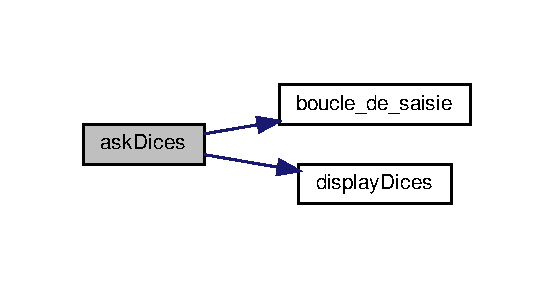
\includegraphics[width=266pt]{mecanismeJeu_8h_a9e4530f74b630f0cfcc27b8bddb34ce8_cgraph}
\end{center}
\end{figure}
Here is the caller graph for this function\+:
\nopagebreak
\begin{figure}[H]
\begin{center}
\leavevmode
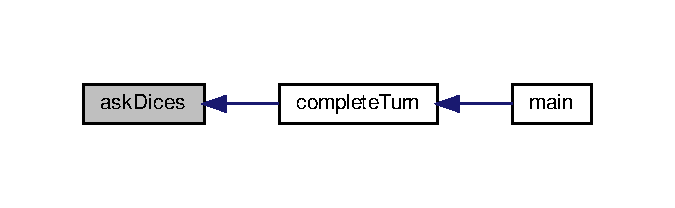
\includegraphics[width=324pt]{mecanismeJeu_8h_a9e4530f74b630f0cfcc27b8bddb34ce8_icgraph}
\end{center}
\end{figure}
\mbox{\Hypertarget{mecanismeJeu_8h_a9ccbcda936f74ce7cb8471cc41b8415e}\label{mecanismeJeu_8h_a9ccbcda936f74ce7cb8471cc41b8415e}} 
\index{mecanisme\+Jeu.\+h@{mecanisme\+Jeu.\+h}!complete\+Turn@{complete\+Turn}}
\index{complete\+Turn@{complete\+Turn}!mecanisme\+Jeu.\+h@{mecanisme\+Jeu.\+h}}
\subsubsection{\texorpdfstring{complete\+Turn()}{completeTurn()}}
{\footnotesize\ttfamily void complete\+Turn (\begin{DoxyParamCaption}\item[{\hyperlink{structPlayer}{Player} $\ast$}]{p }\end{DoxyParamCaption})}



lance une partie de jeu. 

fait une partie de jeu . 
\begin{DoxyParams}{Parameters}
{\em p} & le joueur. \\
\hline
\end{DoxyParams}


Definition at line 94 of file mecanisme\+Jeu.\+c.



References ask\+Dices(), boucle\+\_\+de\+\_\+saisie(), Player\+::dices, display\+Dices(), display\+Score(), display\+Tab\+Score(), Player\+::nbr\+Roll\+Remain, refresh\+Dices(), roll\+Dices(), saisit\+Score(), Player\+::tab\+Score, and Player\+::tab\+Score\+Final.



Referenced by main().


\begin{DoxyCode}
94                             \{
95   \hyperlink{mecanismeJeu_8c_acfee2b60324d906c1d4174e6e51b92d3}{refreshDices}(p) ;
96   \textcolor{keywordtype}{int} answer=1;
97   \textcolor{keywordflow}{do}\{
98     printf(\textcolor{stringliteral}{"Lance de dees :\(\backslash\)n"}) ;
99     \hyperlink{mecanismeJeu_8c_ab55e6b5866c616840bef8cccef4952c5}{rollDices}(p) ;   
100     \hyperlink{mecanismeJeu_8c_ad9ebcce43b3be9b75d300f961d53d329}{displayDices}(p) ;
101     printf(\textcolor{stringliteral}{"Essaies restante : %d\(\backslash\)n"}, p->\hyperlink{structPlayer_ae4c871b61a2af583a8b5975d736bea5d}{nbrRollRemain}) ; 
102     printf(\textcolor{stringliteral}{"Score temporaire :\(\backslash\)n"});
103     \hyperlink{score_8c_a8eab6bc89b1828c4f86d313ad10ecda9}{displayScore}(p->\hyperlink{structPlayer_a7d5c0f37c78c868e4721cc8ceece92a6}{tabScore}, p->\hyperlink{structPlayer_a676bd9687aaa50806f419c4ae170bcb2}{dices},p->\hyperlink{structPlayer_a7c377df37ea43f041207fc4de5ac0a93}{tabScoreFinal});
104 
105     \textcolor{keywordflow}{if}(p->\hyperlink{structPlayer_ae4c871b61a2af583a8b5975d736bea5d}{nbrRollRemain}>0)\{
106 
107         printf(\textcolor{stringliteral}{"Voulez vous relancer des dees ? "}) ;
108         \hyperlink{score_8c_a1e229810418844ae6a50ff60d258d017}{boucle\_de\_saisie}(&answer,0,1) ;
109         \textcolor{keywordflow}{if}(!answer)\{
110             p->\hyperlink{structPlayer_ae4c871b61a2af583a8b5975d736bea5d}{nbrRollRemain} =0;
111         \}
112         \textcolor{keywordflow}{else}\{
113             \hyperlink{mecanismeJeu_8c_a9e4530f74b630f0cfcc27b8bddb34ce8}{askDices}(p);
114         \}
115     \}
116   \}\textcolor{keywordflow}{while}(p->\hyperlink{structPlayer_ae4c871b61a2af583a8b5975d736bea5d}{nbrRollRemain} >= 0);
117 
118     \hyperlink{score_8c_ab920728e54ed8e7c6f0481cd7527ba80}{saisitScore}(p->\hyperlink{structPlayer_a7d5c0f37c78c868e4721cc8ceece92a6}{tabScore},p->\hyperlink{structPlayer_a7c377df37ea43f041207fc4de5ac0a93}{tabScoreFinal});
119     \textcolor{keywordflow}{for} (\textcolor{keywordtype}{int} i = 0; i < 20; ++i)
120     \{
121         printf(\textcolor{stringliteral}{"%d\(\backslash\)n"}, p->\hyperlink{structPlayer_a7c377df37ea43f041207fc4de5ac0a93}{tabScoreFinal}[i] );
122     \}
123 
124   \hyperlink{score_8c_a29ba6e6017af53e5247f75843148f2d1}{displayTabScore}(p->\hyperlink{structPlayer_a7d5c0f37c78c868e4721cc8ceece92a6}{tabScore},p->\hyperlink{structPlayer_a7c377df37ea43f041207fc4de5ac0a93}{tabScoreFinal});\textcolor{comment}{//affiche son score
       final}
125 \}
\end{DoxyCode}
Here is the call graph for this function\+:
\nopagebreak
\begin{figure}[H]
\begin{center}
\leavevmode
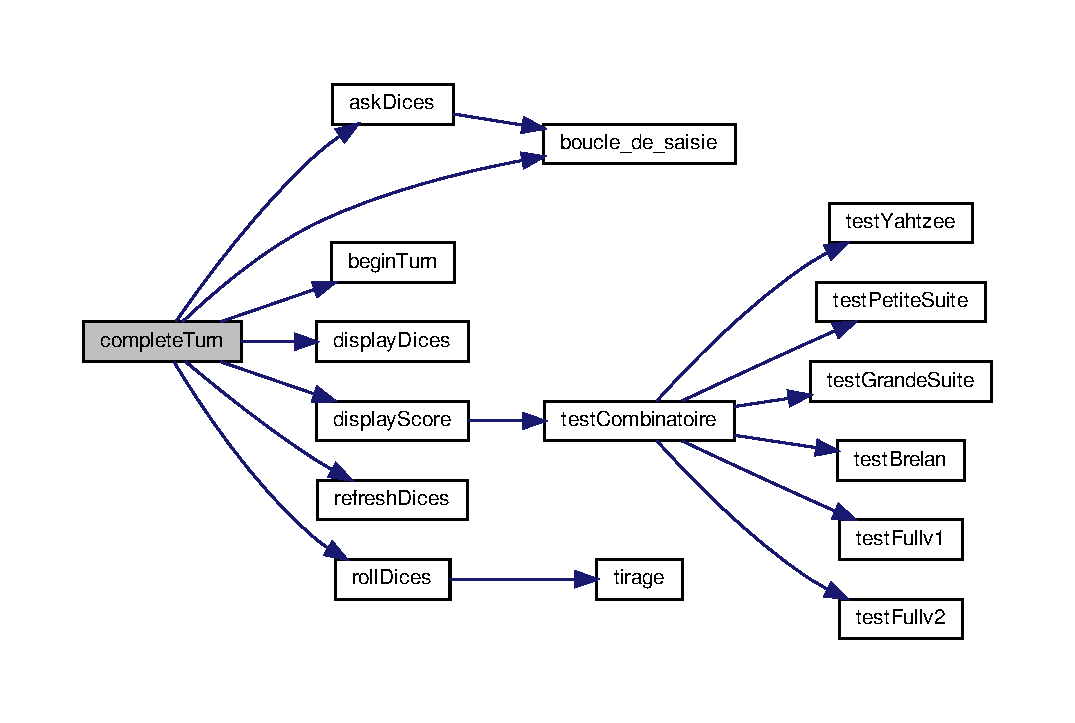
\includegraphics[width=350pt]{mecanismeJeu_8h_a9ccbcda936f74ce7cb8471cc41b8415e_cgraph}
\end{center}
\end{figure}
Here is the caller graph for this function\+:
\nopagebreak
\begin{figure}[H]
\begin{center}
\leavevmode
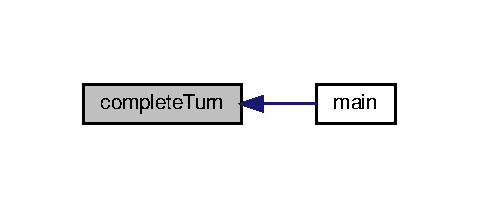
\includegraphics[width=230pt]{mecanismeJeu_8h_a9ccbcda936f74ce7cb8471cc41b8415e_icgraph}
\end{center}
\end{figure}
\mbox{\Hypertarget{mecanismeJeu_8h_ad9ebcce43b3be9b75d300f961d53d329}\label{mecanismeJeu_8h_ad9ebcce43b3be9b75d300f961d53d329}} 
\index{mecanisme\+Jeu.\+h@{mecanisme\+Jeu.\+h}!display\+Dices@{display\+Dices}}
\index{display\+Dices@{display\+Dices}!mecanisme\+Jeu.\+h@{mecanisme\+Jeu.\+h}}
\subsubsection{\texorpdfstring{display\+Dices()}{displayDices()}}
{\footnotesize\ttfamily void display\+Dices (\begin{DoxyParamCaption}\item[{\hyperlink{structPlayer}{Player} $\ast$}]{p }\end{DoxyParamCaption})}



affichage des dées. 

afficher tout les dées. 
\begin{DoxyParams}{Parameters}
{\em p} & le joueur. \\
\hline
\end{DoxyParams}


Definition at line 62 of file mecanisme\+Jeu.\+c.



References Player\+::dices.



Referenced by ask\+Dices(), and complete\+Turn().


\begin{DoxyCode}
62                             \{
63   \textcolor{keywordflow}{for}(\textcolor{keywordtype}{int} i = 0 ; i < 7 ; ++i)\{
64     printf(\textcolor{stringliteral}{"%d "}, p->\hyperlink{structPlayer_a676bd9687aaa50806f419c4ae170bcb2}{dices}[i]) ;
65   \}
66   
67   printf(\textcolor{stringliteral}{"\(\backslash\)n"}) ;
68 \}
\end{DoxyCode}
Here is the caller graph for this function\+:
\nopagebreak
\begin{figure}[H]
\begin{center}
\leavevmode
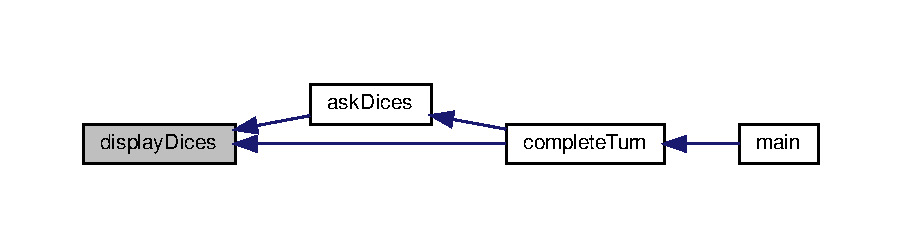
\includegraphics[width=350pt]{mecanismeJeu_8h_ad9ebcce43b3be9b75d300f961d53d329_icgraph}
\end{center}
\end{figure}
\mbox{\Hypertarget{mecanismeJeu_8h_afb996747437467dc9e569a34c469d31b}\label{mecanismeJeu_8h_afb996747437467dc9e569a34c469d31b}} 
\index{mecanisme\+Jeu.\+h@{mecanisme\+Jeu.\+h}!free\+Player@{free\+Player}}
\index{free\+Player@{free\+Player}!mecanisme\+Jeu.\+h@{mecanisme\+Jeu.\+h}}
\subsubsection{\texorpdfstring{free\+Player()}{freePlayer()}}
{\footnotesize\ttfamily void free\+Player (\begin{DoxyParamCaption}\item[{\hyperlink{structPlayer}{Player} $\ast$}]{p }\end{DoxyParamCaption})}



libére la memoire. 

libere la memoire allouer pour les joueurs . 
\begin{DoxyParams}{Parameters}
{\em p} & le joueur. \\
\hline
\end{DoxyParams}


Definition at line 136 of file mecanisme\+Jeu.\+c.



References Player\+::dices, Player\+::dices\+Allowed, Player\+::tab\+Score, and Player\+::tab\+Score\+Final.



Referenced by main().


\begin{DoxyCode}
136                           \{
137         free(p->\hyperlink{structPlayer_a676bd9687aaa50806f419c4ae170bcb2}{dices});
138         free(p->\hyperlink{structPlayer_adb33524b9364f3e0bcfc5bd098cdaaf0}{dicesAllowed});
139         free(p->\hyperlink{structPlayer_a7d5c0f37c78c868e4721cc8ceece92a6}{tabScore});
140         free(p->\hyperlink{structPlayer_a7c377df37ea43f041207fc4de5ac0a93}{tabScoreFinal});
141 \}
\end{DoxyCode}
Here is the caller graph for this function\+:
\nopagebreak
\begin{figure}[H]
\begin{center}
\leavevmode
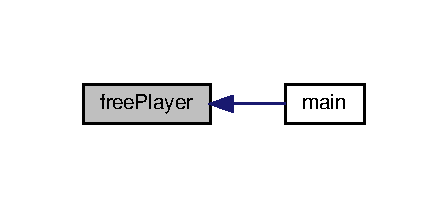
\includegraphics[width=215pt]{mecanismeJeu_8h_afb996747437467dc9e569a34c469d31b_icgraph}
\end{center}
\end{figure}
\mbox{\Hypertarget{mecanismeJeu_8h_acfee2b60324d906c1d4174e6e51b92d3}\label{mecanismeJeu_8h_acfee2b60324d906c1d4174e6e51b92d3}} 
\index{mecanisme\+Jeu.\+h@{mecanisme\+Jeu.\+h}!refresh\+Dices@{refresh\+Dices}}
\index{refresh\+Dices@{refresh\+Dices}!mecanisme\+Jeu.\+h@{mecanisme\+Jeu.\+h}}
\subsubsection{\texorpdfstring{refresh\+Dices()}{refreshDices()}}
{\footnotesize\ttfamily void refresh\+Dices (\begin{DoxyParamCaption}\item[{\hyperlink{structPlayer}{Player} $\ast$}]{p }\end{DoxyParamCaption})}



initialise les dées 

initialize toute les dées a 0. 
\begin{DoxyParams}{Parameters}
{\em p} & le joueur. \\
\hline
\end{DoxyParams}


Definition at line 48 of file mecanisme\+Jeu.\+c.



References Player\+::dices, and Player\+::dices\+Allowed.



Referenced by complete\+Turn().


\begin{DoxyCode}
48                             \{
49 
50   \textcolor{keywordflow}{for}(\textcolor{keywordtype}{int} i = 0 ; i < 7 ; ++i)\{
51     p->\hyperlink{structPlayer_a676bd9687aaa50806f419c4ae170bcb2}{dices}[i] = 0 ;
52     p->\hyperlink{structPlayer_adb33524b9364f3e0bcfc5bd098cdaaf0}{dicesAllowed}[i]=1;
53   \} 
54 \}
\end{DoxyCode}
Here is the caller graph for this function\+:
\nopagebreak
\begin{figure}[H]
\begin{center}
\leavevmode
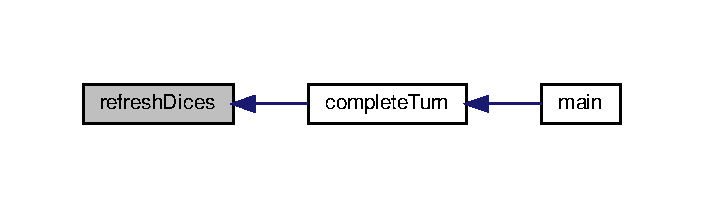
\includegraphics[width=338pt]{mecanismeJeu_8h_acfee2b60324d906c1d4174e6e51b92d3_icgraph}
\end{center}
\end{figure}
\mbox{\Hypertarget{mecanismeJeu_8h_ab55e6b5866c616840bef8cccef4952c5}\label{mecanismeJeu_8h_ab55e6b5866c616840bef8cccef4952c5}} 
\index{mecanisme\+Jeu.\+h@{mecanisme\+Jeu.\+h}!roll\+Dices@{roll\+Dices}}
\index{roll\+Dices@{roll\+Dices}!mecanisme\+Jeu.\+h@{mecanisme\+Jeu.\+h}}
\subsubsection{\texorpdfstring{roll\+Dices()}{rollDices()}}
{\footnotesize\ttfamily void roll\+Dices (\begin{DoxyParamCaption}\item[{\hyperlink{structPlayer}{Player} $\ast$}]{p }\end{DoxyParamCaption})}



la coup de jeu 

fait le coup de 7 deés


\begin{DoxyParams}{Parameters}
{\em p} & le joueur \\
\hline
\end{DoxyParams}


Definition at line 32 of file mecanisme\+Jeu.\+c.



References Player\+::dices, Player\+::dices\+Allowed, Player\+::nbr\+Roll\+Remain, and tirage().



Referenced by complete\+Turn().


\begin{DoxyCode}
32                          \{
33   srand((\textcolor{keywordtype}{unsigned})time(NULL));\textcolor{comment}{//set Seed pour le tirage}
34   \textcolor{keywordflow}{for}(\textcolor{keywordtype}{int} i = 0 ; i < 7; ++i)\{
35     \textcolor{keywordflow}{if} (p->\hyperlink{structPlayer_adb33524b9364f3e0bcfc5bd098cdaaf0}{dicesAllowed}[i])\{
36       p->\hyperlink{structPlayer_a676bd9687aaa50806f419c4ae170bcb2}{dices}[i] = \hyperlink{mecanismeJeu_8c_aedc55fd9756d84e32e3f03e04f964076}{tirage}(8) ;
37       \textcolor{comment}{//printf(">>>de %d tire%d\(\backslash\)n",i,p->dices[i] );}
38     \}
39   \}
40   p->\hyperlink{structPlayer_ae4c871b61a2af583a8b5975d736bea5d}{nbrRollRemain}-=1;
41 \}
\end{DoxyCode}
Here is the call graph for this function\+:
\nopagebreak
\begin{figure}[H]
\begin{center}
\leavevmode
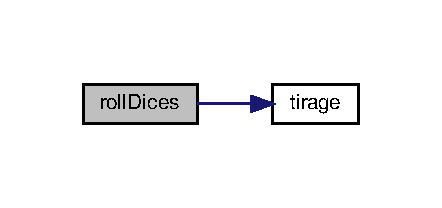
\includegraphics[width=212pt]{mecanismeJeu_8h_ab55e6b5866c616840bef8cccef4952c5_cgraph}
\end{center}
\end{figure}
Here is the caller graph for this function\+:
\nopagebreak
\begin{figure}[H]
\begin{center}
\leavevmode
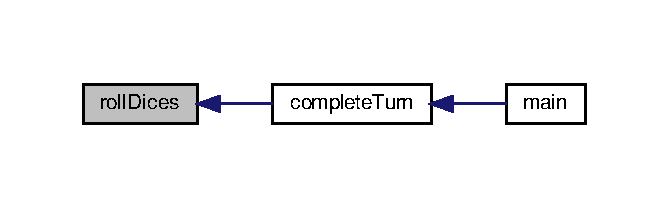
\includegraphics[width=321pt]{mecanismeJeu_8h_ab55e6b5866c616840bef8cccef4952c5_icgraph}
\end{center}
\end{figure}
\mbox{\Hypertarget{mecanismeJeu_8h_aedc55fd9756d84e32e3f03e04f964076}\label{mecanismeJeu_8h_aedc55fd9756d84e32e3f03e04f964076}} 
\index{mecanisme\+Jeu.\+h@{mecanisme\+Jeu.\+h}!tirage@{tirage}}
\index{tirage@{tirage}!mecanisme\+Jeu.\+h@{mecanisme\+Jeu.\+h}}
\subsubsection{\texorpdfstring{tirage()}{tirage()}}
{\footnotesize\ttfamily int tirage (\begin{DoxyParamCaption}\item[{int}]{max }\end{DoxyParamCaption})}



donne la valeur de dée 


\begin{DoxyParams}{Parameters}
{\em max} & le maximum \\
\hline
\end{DoxyParams}
\begin{DoxyReturn}{Returns}
Un int représentant la valeur de dée. 
\end{DoxyReturn}


Definition at line 19 of file mecanisme\+Jeu.\+c.



Referenced by roll\+Dices().


\begin{DoxyCode}
19                    \{
20     \textcolor{comment}{/*tire au sort un nombre compris entre 0 inclus max; }
21 \textcolor{comment}{    srand((unsigned)time(NULL));*/}
22     rand();
23     \textcolor{keywordflow}{return} (\textcolor{keywordtype}{double})(rand()/(double)(RAND\_MAX) * (max))+1;
24 \}
\end{DoxyCode}
Here is the caller graph for this function\+:
\nopagebreak
\begin{figure}[H]
\begin{center}
\leavevmode
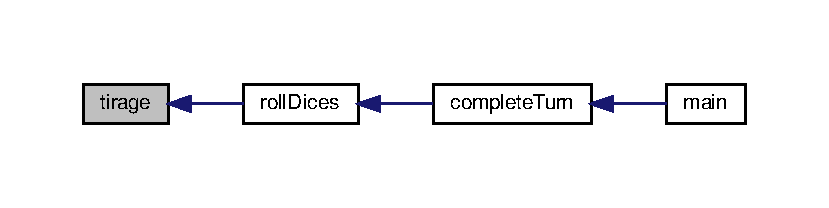
\includegraphics[width=350pt]{mecanismeJeu_8h_aedc55fd9756d84e32e3f03e04f964076_icgraph}
\end{center}
\end{figure}

\hypertarget{proto_8c}{}\section{proto.\+c File Reference}
\label{proto_8c}\index{proto.\+c@{proto.\+c}}
{\ttfamily \#include $<$stdio.\+h$>$}\newline
{\ttfamily \#include $<$stdlib.\+h$>$}\newline
{\ttfamily \#include $<$math.\+h$>$}\newline
{\ttfamily \#include $<$stdarg.\+h$>$}\newline
{\ttfamily \#include \char`\"{}mecanisme\+Jeu.\+h\char`\"{}}\newline
Include dependency graph for proto.\+c\+:\nopagebreak
\begin{figure}[H]
\begin{center}
\leavevmode
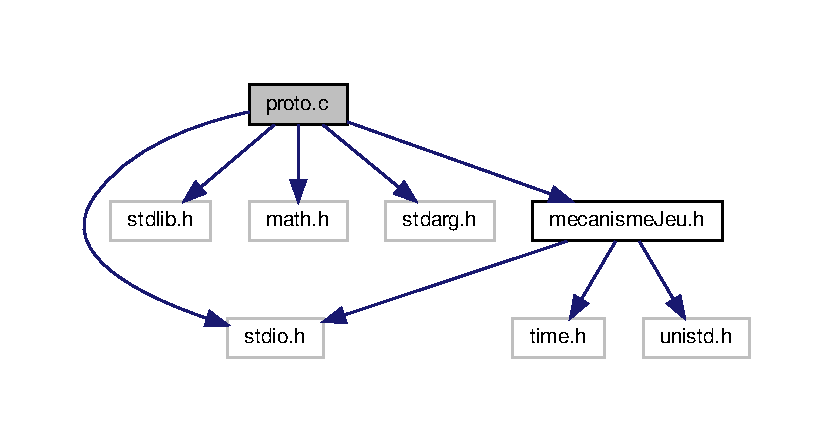
\includegraphics[width=350pt]{proto_8c__incl}
\end{center}
\end{figure}
\subsection*{Functions}
\begin{DoxyCompactItemize}
\item 
int \hyperlink{proto_8c_aedc55fd9756d84e32e3f03e04f964076}{tirage} (int max)
\item 
void \hyperlink{proto_8c_ab55e6b5866c616840bef8cccef4952c5}{roll\+Dices} (\hyperlink{structPlayer}{Player} $\ast$p)
\item 
void \hyperlink{proto_8c_a270db6d766abade9ad6e54cc58e9822b}{begin\+Turn} (\hyperlink{structPlayer}{Player} $\ast$p)
\item 
int \hyperlink{proto_8c_af34915129a343bf4c2718354a681f1fb}{boucle\+\_\+de\+\_\+saisie} (int a, int b)
\item 
void \hyperlink{proto_8c_ad9ebcce43b3be9b75d300f961d53d329}{display\+Dices} (\hyperlink{structPlayer}{Player} $\ast$p)
\item 
void \hyperlink{proto_8c_a9ccbcda936f74ce7cb8471cc41b8415e}{complete\+Turn} (\hyperlink{structPlayer}{Player} $\ast$p)
\item 
int \hyperlink{proto_8c_a840291bc02cba5474a4cb46a9b9566fe}{main} (void)
\end{DoxyCompactItemize}


\subsection{Function Documentation}
\mbox{\Hypertarget{proto_8c_a270db6d766abade9ad6e54cc58e9822b}\label{proto_8c_a270db6d766abade9ad6e54cc58e9822b}} 
\index{proto.\+c@{proto.\+c}!begin\+Turn@{begin\+Turn}}
\index{begin\+Turn@{begin\+Turn}!proto.\+c@{proto.\+c}}
\subsubsection{\texorpdfstring{begin\+Turn()}{beginTurn()}}
{\footnotesize\ttfamily void begin\+Turn (\begin{DoxyParamCaption}\item[{\hyperlink{structPlayer}{Player} $\ast$}]{p }\end{DoxyParamCaption})}



Definition at line 41 of file proto.\+c.



References Player\+::dices, Player\+::dices\+Allowed, and Player\+::nbr\+Roll\+Remain.



Referenced by complete\+Turn().


\begin{DoxyCode}
41                          \{
42 
43   \textcolor{keywordflow}{for}(\textcolor{keywordtype}{int} i = 0 ; i < 6 ; ++i)\{
44     p->\hyperlink{structPlayer_a676bd9687aaa50806f419c4ae170bcb2}{dices}[i] = 0 ;
45     p->\hyperlink{structPlayer_adb33524b9364f3e0bcfc5bd098cdaaf0}{dicesAllowed}[i]=1;
46   \}
47   p->\hyperlink{structPlayer_ae4c871b61a2af583a8b5975d736bea5d}{nbrRollRemain} = 6 ; 
48 \}
\end{DoxyCode}
Here is the caller graph for this function\+:\nopagebreak
\begin{figure}[H]
\begin{center}
\leavevmode
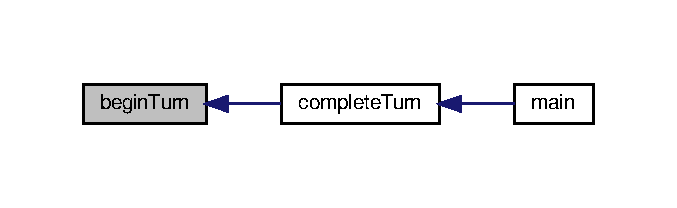
\includegraphics[width=325pt]{proto_8c_a270db6d766abade9ad6e54cc58e9822b_icgraph}
\end{center}
\end{figure}
\mbox{\Hypertarget{proto_8c_af34915129a343bf4c2718354a681f1fb}\label{proto_8c_af34915129a343bf4c2718354a681f1fb}} 
\index{proto.\+c@{proto.\+c}!boucle\+\_\+de\+\_\+saisie@{boucle\+\_\+de\+\_\+saisie}}
\index{boucle\+\_\+de\+\_\+saisie@{boucle\+\_\+de\+\_\+saisie}!proto.\+c@{proto.\+c}}
\subsubsection{\texorpdfstring{boucle\+\_\+de\+\_\+saisie()}{boucle\_de\_saisie()}}
{\footnotesize\ttfamily int boucle\+\_\+de\+\_\+saisie (\begin{DoxyParamCaption}\item[{int}]{a,  }\item[{int}]{b }\end{DoxyParamCaption})}



Definition at line 51 of file proto.\+c.



Referenced by complete\+Turn().


\begin{DoxyCode}
51                                   \{
52     \textcolor{comment}{//retourne l'entier i ssi il est compris dans intervalle [a,b]}
53     \textcolor{keywordtype}{int} i;
54     \textcolor{keywordflow}{do}\{
55         fflush(stdin);
56         \textcolor{comment}{//necessaire pour eviter un bug de boucle infinie si utilisateur saisie un type non int comme une
       charactere par exemple}
57         \textcolor{comment}{//meme si un char est un int...(scanf)}
58         printf(\textcolor{stringliteral}{"merci de saisir un nombre compris entre %d et %d\(\backslash\)n"}, a, b);
59         scanf(\textcolor{stringliteral}{"%d"},&i);
60     \}\textcolor{keywordflow}{while}( i <a || i>b ||\textcolor{keyword}{sizeof}(i) != \textcolor{keyword}{sizeof}(\textcolor{keywordtype}{int}) );
61     \textcolor{keywordflow}{return} i;
62 \}
\end{DoxyCode}
Here is the caller graph for this function\+:\nopagebreak
\begin{figure}[H]
\begin{center}
\leavevmode
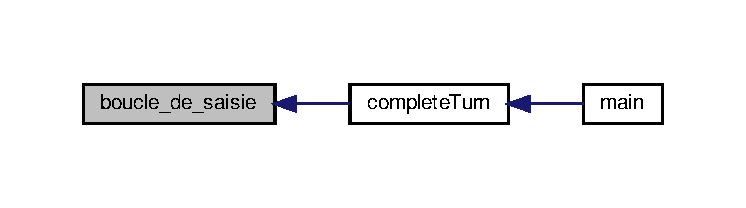
\includegraphics[width=350pt]{proto_8c_af34915129a343bf4c2718354a681f1fb_icgraph}
\end{center}
\end{figure}
\mbox{\Hypertarget{proto_8c_a9ccbcda936f74ce7cb8471cc41b8415e}\label{proto_8c_a9ccbcda936f74ce7cb8471cc41b8415e}} 
\index{proto.\+c@{proto.\+c}!complete\+Turn@{complete\+Turn}}
\index{complete\+Turn@{complete\+Turn}!proto.\+c@{proto.\+c}}
\subsubsection{\texorpdfstring{complete\+Turn()}{completeTurn()}}
{\footnotesize\ttfamily void complete\+Turn (\begin{DoxyParamCaption}\item[{\hyperlink{structPlayer}{Player} $\ast$}]{p }\end{DoxyParamCaption})}



Definition at line 73 of file proto.\+c.



References ask\+Dices(), begin\+Turn(), boucle\+\_\+de\+\_\+saisie(), Player\+::dices, display\+Dices(), display\+Score(), Player\+::nbr\+Roll\+Remain, refresh\+Dices(), roll\+Dices(), and Player\+::tab\+Score.



Referenced by main().


\begin{DoxyCode}
73                             \{
74   \textcolor{keywordtype}{int} v = 1 ;
75   \textcolor{keywordtype}{int} i = 0 ;
76   \hyperlink{proto_8c_a270db6d766abade9ad6e54cc58e9822b}{beginTurn}(p) ;
77   \textcolor{keywordflow}{while}(p->\hyperlink{structPlayer_ae4c871b61a2af583a8b5975d736bea5d}{nbrRollRemain} != 0)\{
78     printf(\textcolor{stringliteral}{"Actual outcome :\(\backslash\)n"}) ;
79     \hyperlink{proto_8c_ad9ebcce43b3be9b75d300f961d53d329}{displayDices}(p) ;
80     printf(\textcolor{stringliteral}{"Retoss some dice ? "}) ;
81     \textcolor{comment}{//scanf("%d", &v) ;}
82     v = \hyperlink{proto_8c_af34915129a343bf4c2718354a681f1fb}{boucle\_de\_saisie}(0,1) ;
83     \textcolor{keywordflow}{if}(v == 0) \{ p->\hyperlink{structPlayer_ae4c871b61a2af583a8b5975d736bea5d}{nbrRollRemain} = 0 ; \} \textcolor{comment}{//TODO appeler l'affichage de la grille}
84     \textcolor{keywordflow}{else}\{
85       
86       \textcolor{keywordtype}{int} roll = 1 ;
87       \textcolor{keywordflow}{while}(roll == 1 && p->\hyperlink{structPlayer_ae4c871b61a2af583a8b5975d736bea5d}{nbrRollRemain} != 0)\{
88     printf(\textcolor{stringliteral}{"Which one ? "}) ;
89     scanf(\textcolor{stringliteral}{"%d"}, &p->wannaRoll[i]) ;
90     ++i ;
91     printf(\textcolor{stringliteral}{"Select one other dice ? "}) ;
92     scanf(\textcolor{stringliteral}{"%d"}, &roll) ;     
93       \}
94       p->\hyperlink{structPlayer_ae4c871b61a2af583a8b5975d736bea5d}{nbrRollRemain} -= 1 ;
95       \hyperlink{proto_8c_ab55e6b5866c616840bef8cccef4952c5}{rollDices}(p) ;
96       printf(\textcolor{stringliteral}{"You've toss %d dice(s) again :\(\backslash\)nOUTCOME\(\backslash\)n"}, i) ;
97       \hyperlink{proto_8c_ad9ebcce43b3be9b75d300f961d53d329}{displayDices}(p) ;
98       printf(\textcolor{stringliteral}{"Remaining try : %d\(\backslash\)n"}, p->\hyperlink{structPlayer_ae4c871b61a2af583a8b5975d736bea5d}{nbrRollRemain}) ; 
99     \}
100   \}
101   printf(\textcolor{stringliteral}{"Next turn\(\backslash\)n"}) ;
102 \}
\end{DoxyCode}
Here is the call graph for this function\+:\nopagebreak
\begin{figure}[H]
\begin{center}
\leavevmode
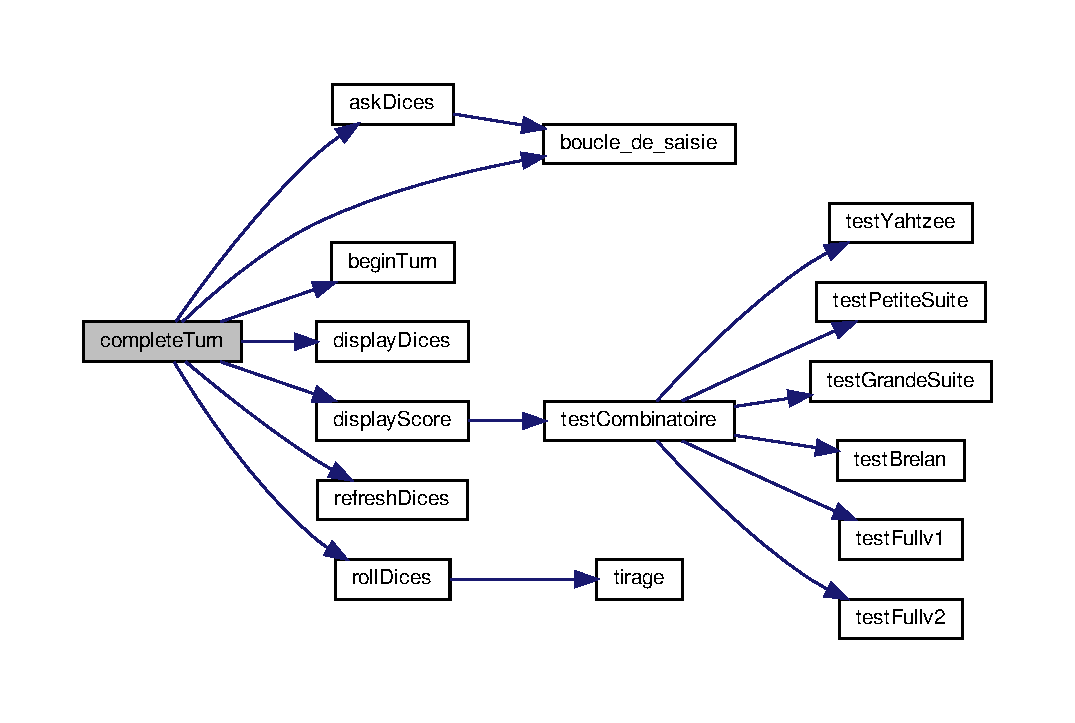
\includegraphics[width=350pt]{proto_8c_a9ccbcda936f74ce7cb8471cc41b8415e_cgraph}
\end{center}
\end{figure}
Here is the caller graph for this function\+:\nopagebreak
\begin{figure}[H]
\begin{center}
\leavevmode
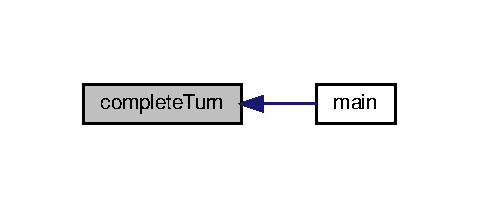
\includegraphics[width=230pt]{proto_8c_a9ccbcda936f74ce7cb8471cc41b8415e_icgraph}
\end{center}
\end{figure}
\mbox{\Hypertarget{proto_8c_ad9ebcce43b3be9b75d300f961d53d329}\label{proto_8c_ad9ebcce43b3be9b75d300f961d53d329}} 
\index{proto.\+c@{proto.\+c}!display\+Dices@{display\+Dices}}
\index{display\+Dices@{display\+Dices}!proto.\+c@{proto.\+c}}
\subsubsection{\texorpdfstring{display\+Dices()}{displayDices()}}
{\footnotesize\ttfamily void display\+Dices (\begin{DoxyParamCaption}\item[{\hyperlink{structPlayer}{Player} $\ast$}]{p }\end{DoxyParamCaption})}



Definition at line 64 of file proto.\+c.



References Player\+::dices.



Referenced by complete\+Turn().


\begin{DoxyCode}
64                             \{
65   \textcolor{keywordflow}{for}(\textcolor{keywordtype}{int} i = 0 ; i < 6 ; ++i)\{
66     printf(\textcolor{stringliteral}{"%d "}, p->\hyperlink{structPlayer_a676bd9687aaa50806f419c4ae170bcb2}{dices}[i]) ;
67     printf(\textcolor{stringliteral}{"... "});
68     sleep(1);
69   \}
70   printf(\textcolor{stringliteral}{"\(\backslash\)n"}) ;
71 \}
\end{DoxyCode}
Here is the caller graph for this function\+:\nopagebreak
\begin{figure}[H]
\begin{center}
\leavevmode
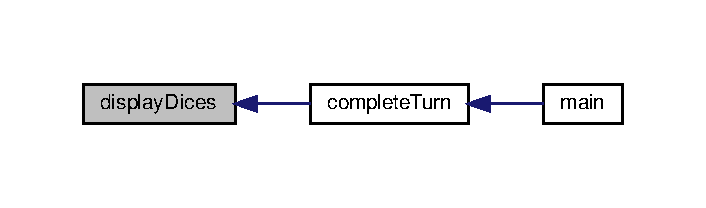
\includegraphics[width=339pt]{proto_8c_ad9ebcce43b3be9b75d300f961d53d329_icgraph}
\end{center}
\end{figure}
\mbox{\Hypertarget{proto_8c_a840291bc02cba5474a4cb46a9b9566fe}\label{proto_8c_a840291bc02cba5474a4cb46a9b9566fe}} 
\index{proto.\+c@{proto.\+c}!main@{main}}
\index{main@{main}!proto.\+c@{proto.\+c}}
\subsubsection{\texorpdfstring{main()}{main()}}
{\footnotesize\ttfamily int main (\begin{DoxyParamCaption}\item[{void}]{ }\end{DoxyParamCaption})}



Definition at line 104 of file proto.\+c.



References complete\+Turn(), and Player\+::dices.


\begin{DoxyCode}
104                \{
105   printf(\textcolor{stringliteral}{"NOTE : répondre par 1 ou 0 aux questions et pour selection des dès leurs indexs [1-7]\(\backslash\)n\(\backslash\)n"}); 
106   \hyperlink{structPlayer}{Player} *p ;
107   \hyperlink{structPlayer}{Player} firstPlayer ;
108   p = &firstPlayer ;
109   p->\hyperlink{structPlayer_a676bd9687aaa50806f419c4ae170bcb2}{dices} = malloc(\textcolor{keyword}{sizeof}(\textcolor{keywordtype}{int}) * 7) ;
110   \textcolor{keywordflow}{if}(p->\hyperlink{structPlayer_a676bd9687aaa50806f419c4ae170bcb2}{dices} == NULL) printf(\textcolor{stringliteral}{"p == Null !\(\backslash\)n"}) ; 
111   \hyperlink{proto_8c_a9ccbcda936f74ce7cb8471cc41b8415e}{completeTurn}(p) ;
112   
113   \textcolor{keywordflow}{return}(0) ;
114 \}
\end{DoxyCode}
Here is the call graph for this function\+:\nopagebreak
\begin{figure}[H]
\begin{center}
\leavevmode
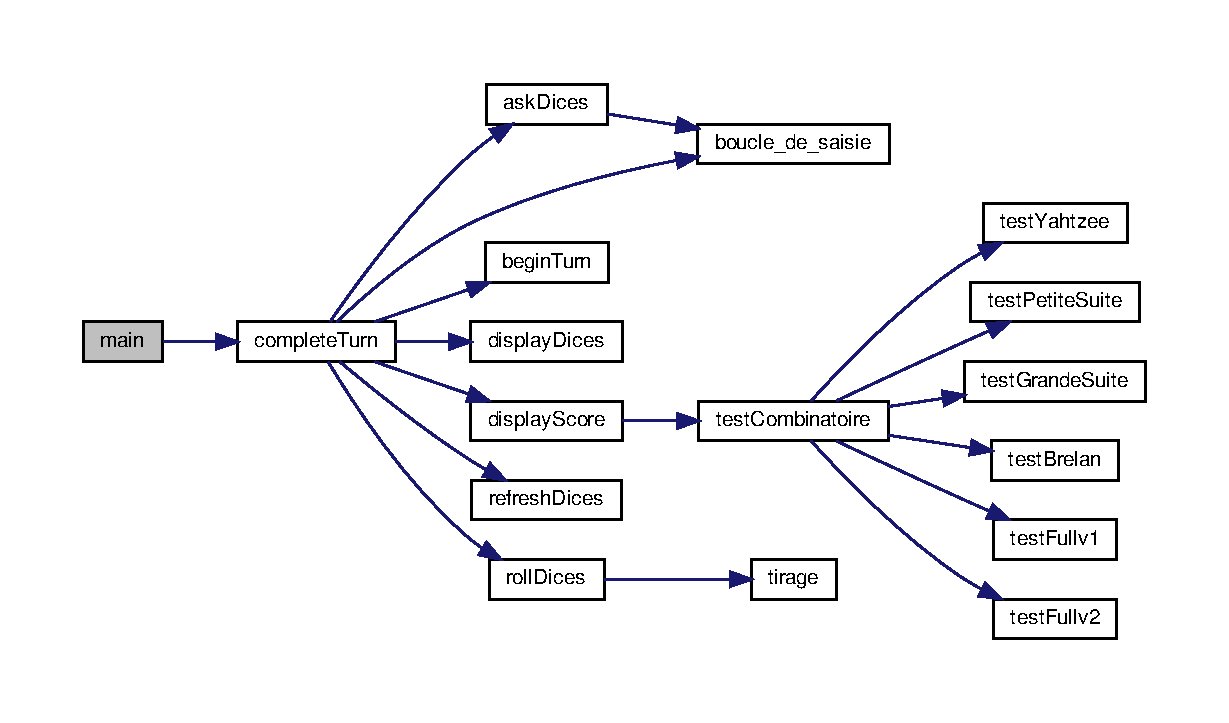
\includegraphics[width=350pt]{proto_8c_a840291bc02cba5474a4cb46a9b9566fe_cgraph}
\end{center}
\end{figure}
\mbox{\Hypertarget{proto_8c_ab55e6b5866c616840bef8cccef4952c5}\label{proto_8c_ab55e6b5866c616840bef8cccef4952c5}} 
\index{proto.\+c@{proto.\+c}!roll\+Dices@{roll\+Dices}}
\index{roll\+Dices@{roll\+Dices}!proto.\+c@{proto.\+c}}
\subsubsection{\texorpdfstring{roll\+Dices()}{rollDices()}}
{\footnotesize\ttfamily void roll\+Dices (\begin{DoxyParamCaption}\item[{\hyperlink{structPlayer}{Player} $\ast$}]{p }\end{DoxyParamCaption})}



Definition at line 31 of file proto.\+c.



References Player\+::dices, and tirage().



Referenced by complete\+Turn().


\begin{DoxyCode}
31                          \{
32   srand((\textcolor{keywordtype}{unsigned})time(NULL));\textcolor{comment}{//set Seed pour le tirage}
33   \textcolor{keywordflow}{for}(\textcolor{keywordtype}{int} i = 0 ; i < 8; ++i)\{
34     \textcolor{comment}{// int sub = va\_arg(va, int) ;}
35     \textcolor{keywordflow}{if} (dicesAllowed[i])\{
36       p->\hyperlink{structPlayer_a676bd9687aaa50806f419c4ae170bcb2}{dices}[p->wannaRoll[i]] = \hyperlink{proto_8c_aedc55fd9756d84e32e3f03e04f964076}{tirage}(8) ;
37     \}
38   \}
39 \}
\end{DoxyCode}
Here is the call graph for this function\+:\nopagebreak
\begin{figure}[H]
\begin{center}
\leavevmode
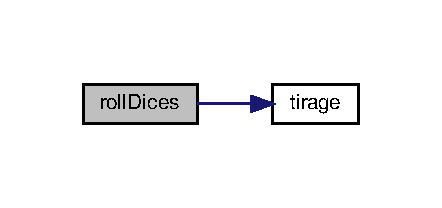
\includegraphics[width=212pt]{proto_8c_ab55e6b5866c616840bef8cccef4952c5_cgraph}
\end{center}
\end{figure}
Here is the caller graph for this function\+:\nopagebreak
\begin{figure}[H]
\begin{center}
\leavevmode
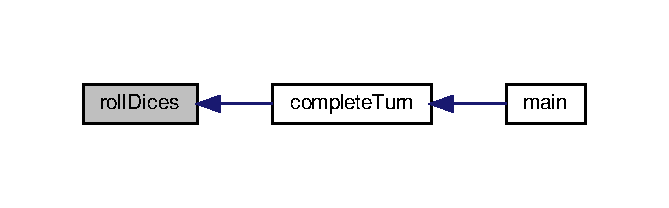
\includegraphics[width=321pt]{proto_8c_ab55e6b5866c616840bef8cccef4952c5_icgraph}
\end{center}
\end{figure}
\mbox{\Hypertarget{proto_8c_aedc55fd9756d84e32e3f03e04f964076}\label{proto_8c_aedc55fd9756d84e32e3f03e04f964076}} 
\index{proto.\+c@{proto.\+c}!tirage@{tirage}}
\index{tirage@{tirage}!proto.\+c@{proto.\+c}}
\subsubsection{\texorpdfstring{tirage()}{tirage()}}
{\footnotesize\ttfamily int tirage (\begin{DoxyParamCaption}\item[{int}]{max }\end{DoxyParamCaption})}



Definition at line 24 of file proto.\+c.



Referenced by roll\+Dices().


\begin{DoxyCode}
24                    \{
25     \textcolor{comment}{/*tire au sort un nombre compris entre 0 inclus max; }
26 \textcolor{comment}{    srand((unsigned)time(NULL));*/}
27     rand();
28     \textcolor{keywordflow}{return} (\textcolor{keywordtype}{double})(rand()/(double)(RAND\_MAX) * (max))+1;
29 \}
\end{DoxyCode}
Here is the caller graph for this function\+:\nopagebreak
\begin{figure}[H]
\begin{center}
\leavevmode
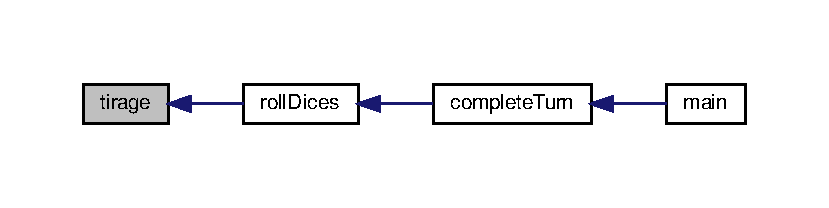
\includegraphics[width=350pt]{proto_8c_aedc55fd9756d84e32e3f03e04f964076_icgraph}
\end{center}
\end{figure}

\hypertarget{README_8md}{}\section{R\+E\+A\+D\+M\+E.\+md File Reference}
\label{README_8md}\index{R\+E\+A\+D\+M\+E.\+md@{R\+E\+A\+D\+M\+E.\+md}}

\hypertarget{score_8c}{}\section{score.\+c File Reference}
\label{score_8c}\index{score.\+c@{score.\+c}}
{\ttfamily \#include \char`\"{}score.\+h\char`\"{}}\newline
Include dependency graph for score.\+c\+:
\nopagebreak
\begin{figure}[H]
\begin{center}
\leavevmode
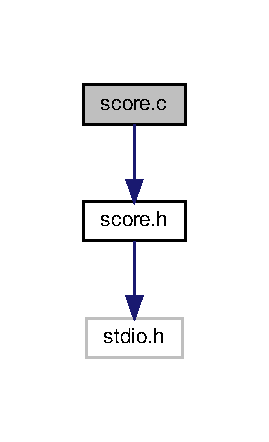
\includegraphics[width=129pt]{score_8c__incl}
\end{center}
\end{figure}
\subsection*{Functions}
\begin{DoxyCompactItemize}
\item 
void \hyperlink{score_8c_a05f60c35ae862a429e026d4410326bd0}{test\+Yahtzee} (int $\ast$tab, int $\ast$tab\+\_\+score)
\item 
void \hyperlink{score_8c_abb5b3478ba11cc275d9e53d024a3842a}{test\+Petite\+Suite} (int $\ast$tab, int $\ast$tab\+\_\+score)
\item 
void \hyperlink{score_8c_a00fb7cc0b89113a887c8cba45a47910a}{test\+Grande\+Suite} (int $\ast$tab, int $\ast$tab\+\_\+score)
\item 
void \hyperlink{score_8c_ab37e17a8d1ec2908a09f6a690ba25388}{test\+Brelan} (int $\ast$tab, int $\ast$tab\+\_\+score)
\item 
void \hyperlink{score_8c_ae2a977f6be696efb8370167ae21268dd}{test\+Fullv1} (int $\ast$tab, int $\ast$tab\+\_\+score)
\item 
void \hyperlink{score_8c_adc172179b41ffc44c1c39c50a4b922e1}{test\+Fullv2} (int $\ast$tab, int $\ast$tab\+\_\+score)
\item 
void \hyperlink{score_8c_a6428b1a4b981622ea3a67b168f1c3c9f}{test\+Combinatoire} (int $\ast$tab\+\_\+score, int $\ast$tab\+\_\+dee)
\item 
void \hyperlink{score_8c_a54d088aca7937ae9e67dabbe160f5254}{display\+Score} (int $\ast$tab\+\_\+score, int $\ast$tab)
\item 
void \hyperlink{score_8c_aeeb20f2b14b47a496fadd754abda5317}{compare\+Score} (int a, int b)
\end{DoxyCompactItemize}


\subsection{Function Documentation}
\mbox{\Hypertarget{score_8c_aeeb20f2b14b47a496fadd754abda5317}\label{score_8c_aeeb20f2b14b47a496fadd754abda5317}} 
\index{score.\+c@{score.\+c}!compare\+Score@{compare\+Score}}
\index{compare\+Score@{compare\+Score}!score.\+c@{score.\+c}}
\subsubsection{\texorpdfstring{compare\+Score()}{compareScore()}}
{\footnotesize\ttfamily void compare\+Score (\begin{DoxyParamCaption}\item[{int}]{a,  }\item[{int}]{b }\end{DoxyParamCaption})}



Definition at line 323 of file score.\+c.



Referenced by main().


\begin{DoxyCode}
323                                \{
324     \textcolor{keywordflow}{if}(a > b)\{
325         printf(\textcolor{stringliteral}{"Bravo! le joueur 1 remporte la partie\(\backslash\)n"});
326     \}
327     \textcolor{keywordflow}{else} \textcolor{keywordflow}{if} (b > a)\{
328         printf(\textcolor{stringliteral}{"Bravo! le joueur 2 remporte la partie\(\backslash\)n"});
329     \}
330     \textcolor{keywordflow}{else}\{
331         printf(\textcolor{stringliteral}{"Match nul\(\backslash\)n"});  
332     \}   
333 \}
\end{DoxyCode}
Here is the caller graph for this function\+:
\nopagebreak
\begin{figure}[H]
\begin{center}
\leavevmode
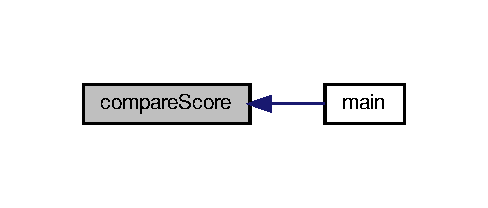
\includegraphics[width=234pt]{score_8c_aeeb20f2b14b47a496fadd754abda5317_icgraph}
\end{center}
\end{figure}
\mbox{\Hypertarget{score_8c_a54d088aca7937ae9e67dabbe160f5254}\label{score_8c_a54d088aca7937ae9e67dabbe160f5254}} 
\index{score.\+c@{score.\+c}!display\+Score@{display\+Score}}
\index{display\+Score@{display\+Score}!score.\+c@{score.\+c}}
\subsubsection{\texorpdfstring{display\+Score()}{displayScore()}}
{\footnotesize\ttfamily void display\+Score (\begin{DoxyParamCaption}\item[{int $\ast$}]{tab\+\_\+score,  }\item[{int $\ast$}]{tab }\end{DoxyParamCaption})}



Definition at line 288 of file score.\+c.



References test\+Combinatoire().



Referenced by complete\+Turn().


\begin{DoxyCode}
288                                           \{
289     \textcolor{keywordtype}{int} i,score=0,somme=0;
290 
291 
292 
293     \hyperlink{score_8c_a6428b1a4b981622ea3a67b168f1c3c9f}{testCombinatoire}(tab\_score,tab);
294 
295     printf(\textcolor{stringliteral}{"voici le score pour Yatzee : %d\(\backslash\)n"},tab\_score[0]);
296            
297     printf(\textcolor{stringliteral}{"voici le score pour Petite Suite : %d\(\backslash\)n"},tab\_score[1]);
298            
299     printf(\textcolor{stringliteral}{"voici le score pour Grande Suite : %d\(\backslash\)n"},tab\_score[2]);
300              
301     printf(\textcolor{stringliteral}{"voici le score pour Brelan : %d\(\backslash\)n"},tab\_score[3]);
302              
303     printf(\textcolor{stringliteral}{"voici le score pour Full : %d\(\backslash\)n"},tab\_score[4]);
304     
305     \textcolor{keywordflow}{for}(i=0;i<8;i++)\{ \textcolor{comment}{// somme de tout les dés}
306       score+=(tab[i]);
307     \}
308 
309     printf(\textcolor{stringliteral}{"voici le score des dés :%d\(\backslash\)n"},score);
310     
311     \textcolor{keywordflow}{for}(i=0;i<5;i++)
312       \{
313         somme+=(tab\_score[i]);
314       \}
315     somme+=score;
316 
317     printf(\textcolor{stringliteral}{"voici le score total : %d\(\backslash\)n"},somme);
318 
319     tab\_score[6] = somme;
320     \}
\end{DoxyCode}
Here is the call graph for this function\+:
\nopagebreak
\begin{figure}[H]
\begin{center}
\leavevmode
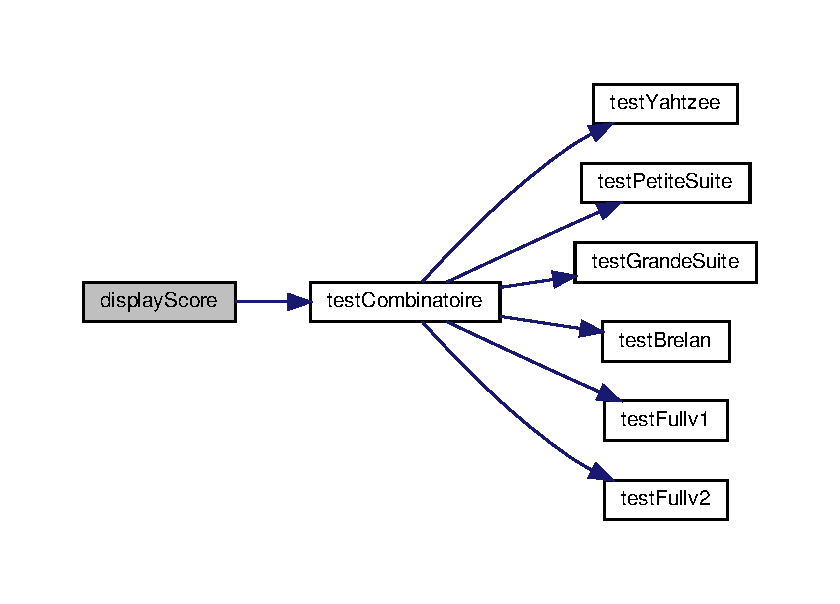
\includegraphics[width=350pt]{score_8c_a54d088aca7937ae9e67dabbe160f5254_cgraph}
\end{center}
\end{figure}
Here is the caller graph for this function\+:
\nopagebreak
\begin{figure}[H]
\begin{center}
\leavevmode
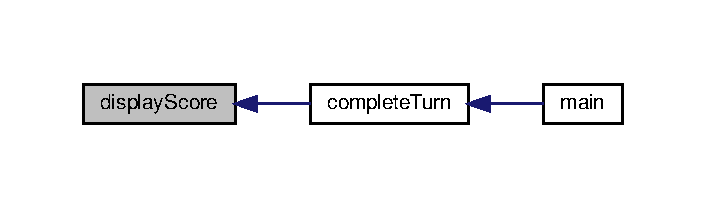
\includegraphics[width=339pt]{score_8c_a54d088aca7937ae9e67dabbe160f5254_icgraph}
\end{center}
\end{figure}
\mbox{\Hypertarget{score_8c_ab37e17a8d1ec2908a09f6a690ba25388}\label{score_8c_ab37e17a8d1ec2908a09f6a690ba25388}} 
\index{score.\+c@{score.\+c}!test\+Brelan@{test\+Brelan}}
\index{test\+Brelan@{test\+Brelan}!score.\+c@{score.\+c}}
\subsubsection{\texorpdfstring{test\+Brelan()}{testBrelan()}}
{\footnotesize\ttfamily void test\+Brelan (\begin{DoxyParamCaption}\item[{int $\ast$}]{tab,  }\item[{int $\ast$}]{tab\+\_\+score }\end{DoxyParamCaption})}



Definition at line 102 of file score.\+c.



Referenced by test\+Combinatoire().


\begin{DoxyCode}
102                                          \{
103   \textcolor{keywordtype}{int} tab\_occurence[8]=\{0,0,0,0,0,0,0\};
104     \textcolor{keywordtype}{int} i,score =0;
105 
106   \textcolor{keywordflow}{for}(i=0;i<8;i++)\{ \textcolor{comment}{// somme de tout les dés}
107     score+=(tab[i]);
108   \}
109 
110   \textcolor{keywordflow}{for}(i=0;i<8;i++) \{
111     
112     \textcolor{keywordflow}{if}(tab[i] == 1)\{
113       tab\_occurence[0]+=1;
114     \}
115     \textcolor{keywordflow}{else} \textcolor{keywordflow}{if}(tab[i] == 2)
116       \{
117     tab\_occurence[1]+=1;
118       \}
119     \textcolor{keywordflow}{else} \textcolor{keywordflow}{if}(tab[i] == 3)
120       \{
121     tab\_occurence[2]+=1;
122       \}
123     \textcolor{keywordflow}{else} \textcolor{keywordflow}{if}(tab[i] == 4)
124       \{
125     tab\_occurence[3]+=1;
126       \}
127     \textcolor{keywordflow}{else} \textcolor{keywordflow}{if}(tab[i] == 5)
128       \{
129     tab\_occurence[4]+=1;
130       \}
131     \textcolor{keywordflow}{else} \textcolor{keywordflow}{if}(tab[i] == 6)
132       \{
133     tab\_occurence[5]+=1;
134       \}
135     \textcolor{keywordflow}{else} \textcolor{keywordflow}{if}(tab[i] == 7)
136       \{
137     tab\_occurence[6]+=1;
138       \}
139     \textcolor{keywordflow}{else} \textcolor{keywordflow}{if}(tab[i] == 8)
140       \{
141     tab\_occurence[7]+=1;
142       \}
143   \}
144     
145     \textcolor{keywordflow}{for}(i=0;i<8;i++)
146       \{
147     \textcolor{keywordflow}{if}(tab\_occurence[i]==3)
148       \{
149         \textcolor{keywordflow}{for}(i=0;i<8;i++)
150           \{
151         \textcolor{keywordflow}{if}(tab\_occurence[i] == 4)
152           \{
153             \textcolor{keywordflow}{return};
154           \}
155           \}
156         tab\_score[3]+=score;
157       \}
158       \}
159 \}
\end{DoxyCode}
Here is the caller graph for this function\+:
\nopagebreak
\begin{figure}[H]
\begin{center}
\leavevmode
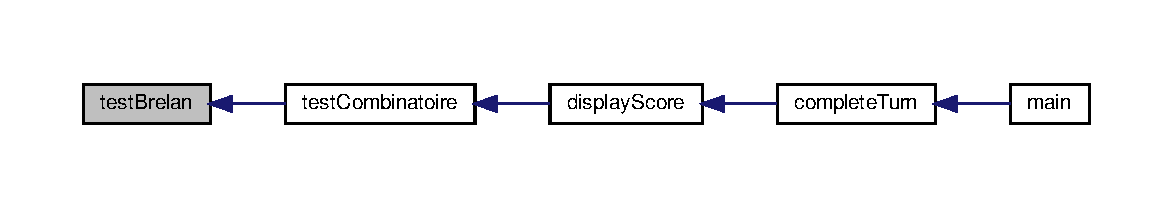
\includegraphics[width=350pt]{score_8c_ab37e17a8d1ec2908a09f6a690ba25388_icgraph}
\end{center}
\end{figure}
\mbox{\Hypertarget{score_8c_a6428b1a4b981622ea3a67b168f1c3c9f}\label{score_8c_a6428b1a4b981622ea3a67b168f1c3c9f}} 
\index{score.\+c@{score.\+c}!test\+Combinatoire@{test\+Combinatoire}}
\index{test\+Combinatoire@{test\+Combinatoire}!score.\+c@{score.\+c}}
\subsubsection{\texorpdfstring{test\+Combinatoire()}{testCombinatoire()}}
{\footnotesize\ttfamily void test\+Combinatoire (\begin{DoxyParamCaption}\item[{int $\ast$}]{tab\+\_\+score,  }\item[{int $\ast$}]{tab\+\_\+dee }\end{DoxyParamCaption})}



Definition at line 275 of file score.\+c.



References test\+Brelan(), test\+Fullv1(), test\+Fullv2(), test\+Grande\+Suite(), test\+Petite\+Suite(), and test\+Yahtzee().



Referenced by display\+Score().


\begin{DoxyCode}
275                                                    \{
276     \textcolor{comment}{/*test et remplit le tableau des score*/}
277     \hyperlink{score_8c_a05f60c35ae862a429e026d4410326bd0}{testYahtzee}(tab\_dee,tab\_score);
278     \hyperlink{score_8c_abb5b3478ba11cc275d9e53d024a3842a}{testPetiteSuite}(tab\_dee,tab\_score);
279     \hyperlink{score_8c_a00fb7cc0b89113a887c8cba45a47910a}{testGrandeSuite}(tab\_dee,tab\_score);
280     \hyperlink{score_8c_ab37e17a8d1ec2908a09f6a690ba25388}{testBrelan}(tab\_dee,tab\_score);
281     \hyperlink{score_8c_ae2a977f6be696efb8370167ae21268dd}{testFullv1}(tab\_dee,tab\_score);
282     \hyperlink{score_8c_adc172179b41ffc44c1c39c50a4b922e1}{testFullv2}(tab\_dee,tab\_score);
283 \}
\end{DoxyCode}
Here is the call graph for this function\+:
\nopagebreak
\begin{figure}[H]
\begin{center}
\leavevmode
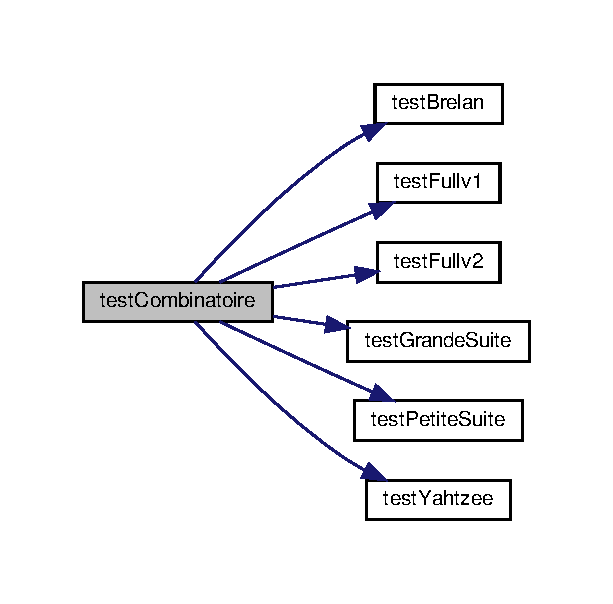
\includegraphics[width=294pt]{score_8c_a6428b1a4b981622ea3a67b168f1c3c9f_cgraph}
\end{center}
\end{figure}
Here is the caller graph for this function\+:
\nopagebreak
\begin{figure}[H]
\begin{center}
\leavevmode
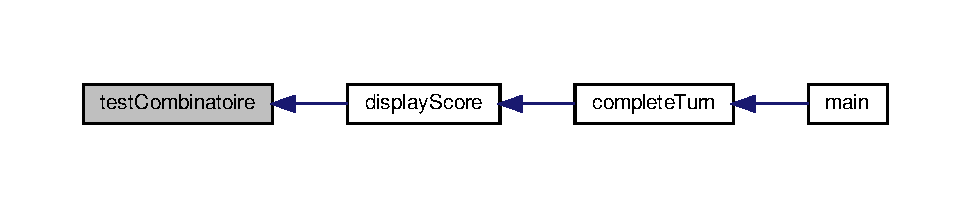
\includegraphics[width=350pt]{score_8c_a6428b1a4b981622ea3a67b168f1c3c9f_icgraph}
\end{center}
\end{figure}
\mbox{\Hypertarget{score_8c_ae2a977f6be696efb8370167ae21268dd}\label{score_8c_ae2a977f6be696efb8370167ae21268dd}} 
\index{score.\+c@{score.\+c}!test\+Fullv1@{test\+Fullv1}}
\index{test\+Fullv1@{test\+Fullv1}!score.\+c@{score.\+c}}
\subsubsection{\texorpdfstring{test\+Fullv1()}{testFullv1()}}
{\footnotesize\ttfamily void test\+Fullv1 (\begin{DoxyParamCaption}\item[{int $\ast$}]{tab,  }\item[{int $\ast$}]{tab\+\_\+score }\end{DoxyParamCaption})}



Definition at line 162 of file score.\+c.



Referenced by test\+Combinatoire().


\begin{DoxyCode}
162                                         \{
163 
164   \textcolor{keywordtype}{int} tab\_occurence[8]=\{0,0,0,0,0,0,0,0\};
165   \textcolor{keywordtype}{int} i,j;
166   \textcolor{keywordflow}{for}(i=0;i<8;i++) \{
167     
168     \textcolor{keywordflow}{if}(tab[i] == 1)\{
169       tab\_occurence[0]+=1;
170     \}
171     \textcolor{keywordflow}{else} \textcolor{keywordflow}{if}(tab[i] == 2)
172       \{
173     tab\_occurence[1]+=1;
174       \}
175     \textcolor{keywordflow}{else} \textcolor{keywordflow}{if}(tab[i] == 3)
176       \{
177     tab\_occurence[2]+=1;
178       \}
179     \textcolor{keywordflow}{else} \textcolor{keywordflow}{if}(tab[i] == 4)
180       \{
181     tab\_occurence[3]+=1;
182       \}
183     \textcolor{keywordflow}{else} \textcolor{keywordflow}{if}(tab[i] == 5)
184       \{
185     tab\_occurence[4]+=1;
186       \}
187     \textcolor{keywordflow}{else} \textcolor{keywordflow}{if}(tab[i] == 6)
188       \{
189     tab\_occurence[5]+=1;
190       \}
191     \textcolor{keywordflow}{else} \textcolor{keywordflow}{if}(tab[i] == 7)
192       \{
193     tab\_occurence[6]+=1;
194       \}
195     \textcolor{keywordflow}{else} \textcolor{keywordflow}{if}(tab[i] == 8)
196       \{
197     tab\_occurence[7]+=1;
198       \}
199   \}
200     
201     \textcolor{keywordflow}{for}(i=0;i<8;i++)
202       \{
203     \textcolor{keywordflow}{if}(tab\_occurence[i]==5)
204       \{
205         \textcolor{keywordflow}{for}(j=0;j<8;j++)
206           \{
207         \textcolor{keywordflow}{if}(tab\_occurence[j]==2)
208           \{
209             tab\_score[4]+=25;           
210           \}
211           \}
212       \}
213       \}
214     
215 \}
\end{DoxyCode}
Here is the caller graph for this function\+:
\nopagebreak
\begin{figure}[H]
\begin{center}
\leavevmode
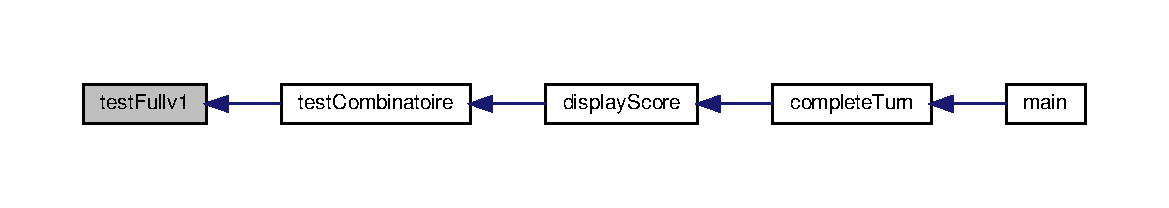
\includegraphics[width=350pt]{score_8c_ae2a977f6be696efb8370167ae21268dd_icgraph}
\end{center}
\end{figure}
\mbox{\Hypertarget{score_8c_adc172179b41ffc44c1c39c50a4b922e1}\label{score_8c_adc172179b41ffc44c1c39c50a4b922e1}} 
\index{score.\+c@{score.\+c}!test\+Fullv2@{test\+Fullv2}}
\index{test\+Fullv2@{test\+Fullv2}!score.\+c@{score.\+c}}
\subsubsection{\texorpdfstring{test\+Fullv2()}{testFullv2()}}
{\footnotesize\ttfamily void test\+Fullv2 (\begin{DoxyParamCaption}\item[{int $\ast$}]{tab,  }\item[{int $\ast$}]{tab\+\_\+score }\end{DoxyParamCaption})}



Definition at line 218 of file score.\+c.



Referenced by test\+Combinatoire().


\begin{DoxyCode}
218                                         \{
219   \textcolor{keywordtype}{int} tab\_occurence[8]=\{0,0,0,0,0,0,0,0\};
220 
221   \textcolor{keywordtype}{int} i,j;
222   \textcolor{keywordflow}{for}(i=0;i<8;i++) \{
223     
224     \textcolor{keywordflow}{if}(tab[i] == 1)\{
225       tab\_occurence[0]+=1;
226     \}
227     \textcolor{keywordflow}{else} \textcolor{keywordflow}{if}(tab[i] == 2)
228       \{
229     tab\_occurence[1]+=1;
230       \}
231     \textcolor{keywordflow}{else} \textcolor{keywordflow}{if}(tab[i] == 3)
232       \{
233     tab\_occurence[2]+=1;
234       \}
235     \textcolor{keywordflow}{else} \textcolor{keywordflow}{if}(tab[i] == 4)
236       \{
237     tab\_occurence[3]+=1;
238       \}
239     \textcolor{keywordflow}{else} \textcolor{keywordflow}{if}(tab[i] == 5)
240       \{
241     tab\_occurence[4]+=1;
242       \}
243     \textcolor{keywordflow}{else} \textcolor{keywordflow}{if}(tab[i] == 6)
244       \{
245     tab\_occurence[5]+=1;
246       \}
247     \textcolor{keywordflow}{else} \textcolor{keywordflow}{if}(tab[i] == 7)
248       \{
249     tab\_occurence[6]+=1;
250       \}
251     \textcolor{keywordflow}{else} \textcolor{keywordflow}{if}(tab[i] == 8)
252       \{
253     tab\_occurence[7]+=1;
254       \}
255   \}
256     
257     \textcolor{keywordflow}{for}(i=0;i<8;i++)
258       \{
259     \textcolor{keywordflow}{if}(tab\_occurence[i]==3)
260       \{
261         \textcolor{keywordflow}{for}(j=0;j<8;j++)
262           \{
263         \textcolor{keywordflow}{if}(tab\_occurence[j]==4)
264           \{
265 
266             tab\_score[4]+=25;           
267 
268           \}
269           \}
270       \}
271       \}
272     
273 \}
\end{DoxyCode}
Here is the caller graph for this function\+:
\nopagebreak
\begin{figure}[H]
\begin{center}
\leavevmode
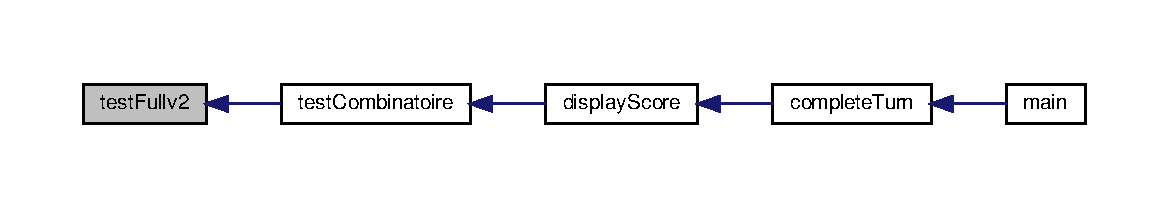
\includegraphics[width=350pt]{score_8c_adc172179b41ffc44c1c39c50a4b922e1_icgraph}
\end{center}
\end{figure}
\mbox{\Hypertarget{score_8c_a00fb7cc0b89113a887c8cba45a47910a}\label{score_8c_a00fb7cc0b89113a887c8cba45a47910a}} 
\index{score.\+c@{score.\+c}!test\+Grande\+Suite@{test\+Grande\+Suite}}
\index{test\+Grande\+Suite@{test\+Grande\+Suite}!score.\+c@{score.\+c}}
\subsubsection{\texorpdfstring{test\+Grande\+Suite()}{testGrandeSuite()}}
{\footnotesize\ttfamily void test\+Grande\+Suite (\begin{DoxyParamCaption}\item[{int $\ast$}]{tab,  }\item[{int $\ast$}]{tab\+\_\+score }\end{DoxyParamCaption})}



Definition at line 60 of file score.\+c.



Referenced by test\+Combinatoire().


\begin{DoxyCode}
60                                               \{
61     \textcolor{keywordtype}{int} i;
62     
63   \textcolor{comment}{// verif grande suite}
64    \textcolor{keywordflow}{for}(i=0;i<8;i++)\{
65         \textcolor{keywordflow}{if}(tab[i] == 2)
66       \{
67         \textcolor{keywordflow}{for}(i=0;i<8;i++)\{
68           \textcolor{keywordflow}{if}(tab[i] == 3)
69          \{
70            \textcolor{keywordflow}{for}(i=0;i<8;i++)\{
71              \textcolor{keywordflow}{if}(tab[i] == 4)
72                 \{
73               \textcolor{keywordflow}{for}(i=0;i<8;i++)\{
74                 \textcolor{keywordflow}{if}(tab[i] == 5)
75                    \{
76                  \textcolor{keywordflow}{for}(i=0;i<8;i++)\{
77                    \textcolor{keywordflow}{if}(tab[i] == 6)
78                       \{
79                     \textcolor{keywordflow}{for}(i=0;i<8;i++)\{
80                       \textcolor{keywordflow}{if}(tab[i] == 7)
81                          \{
82                            \textcolor{keywordflow}{for}(i=0;i<8;i++)\{
83                          \textcolor{keywordflow}{if}(tab[i] == 8)
84                            \{
85                              tab\_score[2]+=40;
86                            \}
87                            \}
88                          \}
89                     \}
90                       \}
91                  \}
92                    \}
93               \}
94             \}
95            \}
96          \}
97         \}
98       \}
99    \}
100    \}
\end{DoxyCode}
Here is the caller graph for this function\+:
\nopagebreak
\begin{figure}[H]
\begin{center}
\leavevmode
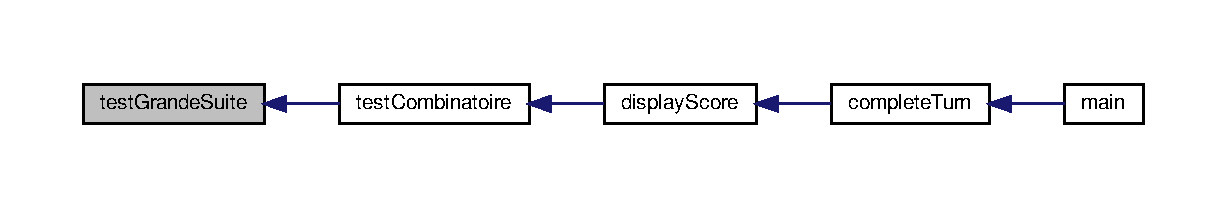
\includegraphics[width=350pt]{score_8c_a00fb7cc0b89113a887c8cba45a47910a_icgraph}
\end{center}
\end{figure}
\mbox{\Hypertarget{score_8c_abb5b3478ba11cc275d9e53d024a3842a}\label{score_8c_abb5b3478ba11cc275d9e53d024a3842a}} 
\index{score.\+c@{score.\+c}!test\+Petite\+Suite@{test\+Petite\+Suite}}
\index{test\+Petite\+Suite@{test\+Petite\+Suite}!score.\+c@{score.\+c}}
\subsubsection{\texorpdfstring{test\+Petite\+Suite()}{testPetiteSuite()}}
{\footnotesize\ttfamily void test\+Petite\+Suite (\begin{DoxyParamCaption}\item[{int $\ast$}]{tab,  }\item[{int $\ast$}]{tab\+\_\+score }\end{DoxyParamCaption})}



Definition at line 20 of file score.\+c.



Referenced by test\+Combinatoire().


\begin{DoxyCode}
20                                               \{
21     \textcolor{keywordtype}{int} i;
22     \textcolor{comment}{// verif petite suite}
23   \textcolor{keywordflow}{for}(i=0;i<8;i++)\{
24         \textcolor{keywordflow}{if}(tab[i] == 1)
25       \{
26         \textcolor{keywordflow}{for}(i=0;i<8;i++)\{
27           \textcolor{keywordflow}{if}(tab[i] == 2)
28          \{
29            \textcolor{keywordflow}{for}(i=0;i<8;i++)\{
30              \textcolor{keywordflow}{if}(tab[i] == 3)
31                 \{
32               \textcolor{keywordflow}{for}(i=0;i<8;i++)\{
33                 \textcolor{keywordflow}{if}(tab[i] == 4)
34                    \{
35                  \textcolor{keywordflow}{for}(i=0;i<8;i++)\{
36                    \textcolor{keywordflow}{if}(tab[i] == 5)
37                       \{
38                     \textcolor{keywordflow}{for}(i=0;i<8;i++)\{
39                       \textcolor{keywordflow}{if}(tab[i] == 6)
40                          \{
41                            \textcolor{keywordflow}{for}(i=0;i<8;i++)\{
42                          \textcolor{keywordflow}{if}(tab[i] == 7)
43                            \{                                                   tab\_score[1]+=30;
44                            \}
45                            \}
46                          \}
47                     \}
48                       \}
49                  \}
50                    \}
51               \}
52             \}
53            \}
54          \}
55         \}
56       \}
57   \}
58   \}
\end{DoxyCode}
Here is the caller graph for this function\+:
\nopagebreak
\begin{figure}[H]
\begin{center}
\leavevmode
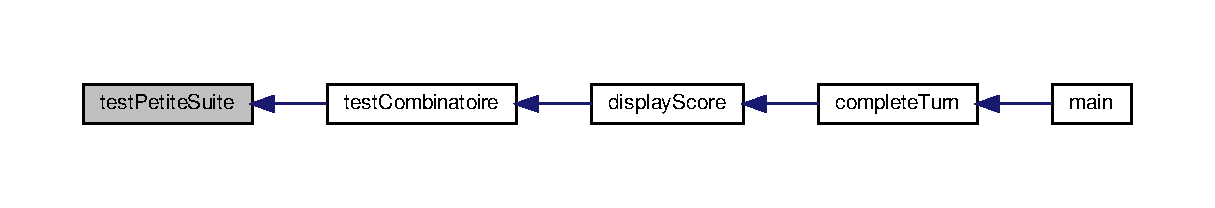
\includegraphics[width=350pt]{score_8c_abb5b3478ba11cc275d9e53d024a3842a_icgraph}
\end{center}
\end{figure}
\mbox{\Hypertarget{score_8c_a05f60c35ae862a429e026d4410326bd0}\label{score_8c_a05f60c35ae862a429e026d4410326bd0}} 
\index{score.\+c@{score.\+c}!test\+Yahtzee@{test\+Yahtzee}}
\index{test\+Yahtzee@{test\+Yahtzee}!score.\+c@{score.\+c}}
\subsubsection{\texorpdfstring{test\+Yahtzee()}{testYahtzee()}}
{\footnotesize\ttfamily void test\+Yahtzee (\begin{DoxyParamCaption}\item[{int $\ast$}]{tab,  }\item[{int $\ast$}]{tab\+\_\+score }\end{DoxyParamCaption})}



Definition at line 3 of file score.\+c.



Referenced by test\+Combinatoire().


\begin{DoxyCode}
3                                           \{
4   \textcolor{comment}{// verif Yahtzee}
5   \textcolor{keywordflow}{if}(tab[0] == tab[1]) \{
6     \textcolor{keywordflow}{if}(tab[1] == tab[2]) \{
7       \textcolor{keywordflow}{if}(tab[2] == tab[3]) \{
8     \textcolor{keywordflow}{if}(tab[3] == tab[4]) \{
9       \textcolor{keywordflow}{if}(tab[4] == tab[5]) \{
10         \textcolor{keywordflow}{if}(tab[5] == tab[6]) \{
11         tab\_score[0]+= 50;
12           \}
13           \}
14       \}
15     \}
16       \}
17     \}
18 \}
\end{DoxyCode}
Here is the caller graph for this function\+:
\nopagebreak
\begin{figure}[H]
\begin{center}
\leavevmode
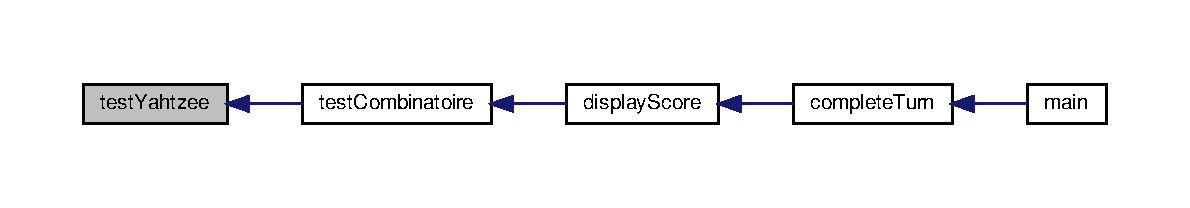
\includegraphics[width=350pt]{score_8c_a05f60c35ae862a429e026d4410326bd0_icgraph}
\end{center}
\end{figure}

\hypertarget{score_8h}{}\section{score.\+h File Reference}
\label{score_8h}\index{score.\+h@{score.\+h}}
{\ttfamily \#include $<$stdio.\+h$>$}\newline
Include dependency graph for score.\+h\+:
\nopagebreak
\begin{figure}[H]
\begin{center}
\leavevmode
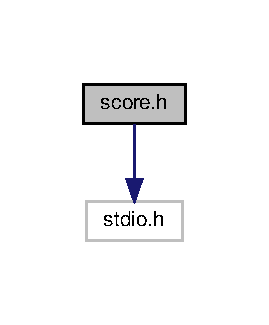
\includegraphics[width=129pt]{score_8h__incl}
\end{center}
\end{figure}
This graph shows which files directly or indirectly include this file\+:
\nopagebreak
\begin{figure}[H]
\begin{center}
\leavevmode
\includegraphics[width=303pt]{score_8h__dep__incl}
\end{center}
\end{figure}
\subsection*{Functions}
\begin{DoxyCompactItemize}
\item 
void \hyperlink{score_8h_a54d088aca7937ae9e67dabbe160f5254}{display\+Score} (int $\ast$tab\+\_\+score, int $\ast$tab)
\item 
void \hyperlink{score_8h_aeeb20f2b14b47a496fadd754abda5317}{compare\+Score} (int a, int b)
\end{DoxyCompactItemize}


\subsection{Function Documentation}
\mbox{\Hypertarget{score_8h_aeeb20f2b14b47a496fadd754abda5317}\label{score_8h_aeeb20f2b14b47a496fadd754abda5317}} 
\index{score.\+h@{score.\+h}!compare\+Score@{compare\+Score}}
\index{compare\+Score@{compare\+Score}!score.\+h@{score.\+h}}
\subsubsection{\texorpdfstring{compare\+Score()}{compareScore()}}
{\footnotesize\ttfamily void compare\+Score (\begin{DoxyParamCaption}\item[{int}]{a,  }\item[{int}]{b }\end{DoxyParamCaption})}



Definition at line 323 of file score.\+c.



Referenced by main().


\begin{DoxyCode}
323                                \{
324     \textcolor{keywordflow}{if}(a > b)\{
325         printf(\textcolor{stringliteral}{"Bravo! le joueur 1 remporte la partie\(\backslash\)n"});
326     \}
327     \textcolor{keywordflow}{else} \textcolor{keywordflow}{if} (b > a)\{
328         printf(\textcolor{stringliteral}{"Bravo! le joueur 2 remporte la partie\(\backslash\)n"});
329     \}
330     \textcolor{keywordflow}{else}\{
331         printf(\textcolor{stringliteral}{"Match nul\(\backslash\)n"});  
332     \}   
333 \}
\end{DoxyCode}
Here is the caller graph for this function\+:
\nopagebreak
\begin{figure}[H]
\begin{center}
\leavevmode
\includegraphics[width=234pt]{score_8h_aeeb20f2b14b47a496fadd754abda5317_icgraph}
\end{center}
\end{figure}
\mbox{\Hypertarget{score_8h_a54d088aca7937ae9e67dabbe160f5254}\label{score_8h_a54d088aca7937ae9e67dabbe160f5254}} 
\index{score.\+h@{score.\+h}!display\+Score@{display\+Score}}
\index{display\+Score@{display\+Score}!score.\+h@{score.\+h}}
\subsubsection{\texorpdfstring{display\+Score()}{displayScore()}}
{\footnotesize\ttfamily void display\+Score (\begin{DoxyParamCaption}\item[{int $\ast$}]{tab\+\_\+score,  }\item[{int $\ast$}]{tab }\end{DoxyParamCaption})}



Definition at line 288 of file score.\+c.



References test\+Combinatoire().



Referenced by complete\+Turn().


\begin{DoxyCode}
288                                           \{
289     \textcolor{keywordtype}{int} i,score=0,somme=0;
290 
291 
292 
293     \hyperlink{score_8c_a6428b1a4b981622ea3a67b168f1c3c9f}{testCombinatoire}(tab\_score,tab);
294 
295     printf(\textcolor{stringliteral}{"voici le score pour Yatzee : %d\(\backslash\)n"},tab\_score[0]);
296            
297     printf(\textcolor{stringliteral}{"voici le score pour Petite Suite : %d\(\backslash\)n"},tab\_score[1]);
298            
299     printf(\textcolor{stringliteral}{"voici le score pour Grande Suite : %d\(\backslash\)n"},tab\_score[2]);
300              
301     printf(\textcolor{stringliteral}{"voici le score pour Brelan : %d\(\backslash\)n"},tab\_score[3]);
302              
303     printf(\textcolor{stringliteral}{"voici le score pour Full : %d\(\backslash\)n"},tab\_score[4]);
304     
305     \textcolor{keywordflow}{for}(i=0;i<8;i++)\{ \textcolor{comment}{// somme de tout les dés}
306       score+=(tab[i]);
307     \}
308 
309     printf(\textcolor{stringliteral}{"voici le score des dés :%d\(\backslash\)n"},score);
310     
311     \textcolor{keywordflow}{for}(i=0;i<5;i++)
312       \{
313         somme+=(tab\_score[i]);
314       \}
315     somme+=score;
316 
317     printf(\textcolor{stringliteral}{"voici le score total : %d\(\backslash\)n"},somme);
318 
319     tab\_score[6] = somme;
320     \}
\end{DoxyCode}
Here is the call graph for this function\+:
\nopagebreak
\begin{figure}[H]
\begin{center}
\leavevmode
\includegraphics[width=350pt]{score_8h_a54d088aca7937ae9e67dabbe160f5254_cgraph}
\end{center}
\end{figure}
Here is the caller graph for this function\+:
\nopagebreak
\begin{figure}[H]
\begin{center}
\leavevmode
\includegraphics[width=339pt]{score_8h_a54d088aca7937ae9e67dabbe160f5254_icgraph}
\end{center}
\end{figure}

\hypertarget{yahtzee_8c}{}\section{yahtzee.\+c File Reference}
\label{yahtzee_8c}\index{yahtzee.\+c@{yahtzee.\+c}}
{\ttfamily \#include $<$stdio.\+h$>$}\newline
Include dependency graph for yahtzee.\+c\+:
\nopagebreak
\begin{figure}[H]
\begin{center}
\leavevmode
\includegraphics[width=139pt]{yahtzee_8c__incl}
\end{center}
\end{figure}
\subsection*{Functions}
\begin{DoxyCompactItemize}
\item 
void \hyperlink{yahtzee_8c_a3cbcb012eb71dfe1f8dd190189cffe91}{coup} (int n)
\item 
void \hyperlink{yahtzee_8c_acc94c07260217204c7e0fa62a02dea7f}{remplirtab} (int nbr)
\item 
int \hyperlink{yahtzee_8c_ae66f6b31b5ad750f1fe042a706a4e3d4}{main} ()
\end{DoxyCompactItemize}


\subsection{Function Documentation}
\mbox{\Hypertarget{yahtzee_8c_a3cbcb012eb71dfe1f8dd190189cffe91}\label{yahtzee_8c_a3cbcb012eb71dfe1f8dd190189cffe91}} 
\index{yahtzee.\+c@{yahtzee.\+c}!coup@{coup}}
\index{coup@{coup}!yahtzee.\+c@{yahtzee.\+c}}
\subsubsection{\texorpdfstring{coup()}{coup()}}
{\footnotesize\ttfamily void coup (\begin{DoxyParamCaption}\item[{int}]{n }\end{DoxyParamCaption})}



Definition at line 3 of file yahtzee.\+c.



Referenced by remplirtab().


\begin{DoxyCode}
3                 \{
4   \textcolor{keywordflow}{return} rand() % n;
5 \}
\end{DoxyCode}
Here is the caller graph for this function\+:
\nopagebreak
\begin{figure}[H]
\begin{center}
\leavevmode
\includegraphics[width=213pt]{yahtzee_8c_a3cbcb012eb71dfe1f8dd190189cffe91_icgraph}
\end{center}
\end{figure}
\mbox{\Hypertarget{yahtzee_8c_ae66f6b31b5ad750f1fe042a706a4e3d4}\label{yahtzee_8c_ae66f6b31b5ad750f1fe042a706a4e3d4}} 
\index{yahtzee.\+c@{yahtzee.\+c}!main@{main}}
\index{main@{main}!yahtzee.\+c@{yahtzee.\+c}}
\subsubsection{\texorpdfstring{main()}{main()}}
{\footnotesize\ttfamily int main (\begin{DoxyParamCaption}\item[{void}]{ }\end{DoxyParamCaption})}



Definition at line 15 of file yahtzee.\+c.


\begin{DoxyCode}
15           \{
16 
17   
18   \textcolor{keywordflow}{return} 0;
19 \}
\end{DoxyCode}
\mbox{\Hypertarget{yahtzee_8c_acc94c07260217204c7e0fa62a02dea7f}\label{yahtzee_8c_acc94c07260217204c7e0fa62a02dea7f}} 
\index{yahtzee.\+c@{yahtzee.\+c}!remplirtab@{remplirtab}}
\index{remplirtab@{remplirtab}!yahtzee.\+c@{yahtzee.\+c}}
\subsubsection{\texorpdfstring{remplirtab()}{remplirtab()}}
{\footnotesize\ttfamily void remplirtab (\begin{DoxyParamCaption}\item[{int}]{nbr }\end{DoxyParamCaption})}



Definition at line 7 of file yahtzee.\+c.



References coup().


\begin{DoxyCode}
7                         \{
8   \textcolor{keywordtype}{int} i;
9   \textcolor{keywordflow}{for} (i=0;i<nbr;i++)\{
10     tab[i]=\hyperlink{yahtzee_8c_a3cbcb012eb71dfe1f8dd190189cffe91}{coup}(8);
11   \}
12 \}
\end{DoxyCode}
Here is the call graph for this function\+:
\nopagebreak
\begin{figure}[H]
\begin{center}
\leavevmode
\includegraphics[width=213pt]{yahtzee_8c_acc94c07260217204c7e0fa62a02dea7f_cgraph}
\end{center}
\end{figure}

%--- End generated contents ---

% Index
\backmatter
\newpage
\phantomsection
\clearemptydoublepage
\addcontentsline{toc}{chapter}{Index}
\printindex

\end{document}
